\documentclass[twocolumn,a4paper,10pt]{article}
\usepackage[margin=1in]{geometry}
\usepackage{cite}
\usepackage{amsmath,amssymb,amsfonts}
\usepackage{graphicx}
\usepackage{xcolor}
\usepackage{booktabs}
\usepackage{tabularx}
\usepackage{makecell}

\usepackage{cuted}
\usepackage{caption} % <--- Adds support for \captionof

\usepackage{listings}
\usepackage{xcolor}
\usepackage{float}

\usepackage[htt]{hyphenat}
\lstdefinelanguage{YAML}{
  keywords={true,false,null,y,n},
  keywordstyle=\color{blue},
  sensitive=false,
  comment=[l]{\#},
  morecomment=[s]{/*}{*/},
  commentstyle=\color{gray}\ttfamily,
  stringstyle=\color{purple}\ttfamily,
  moredelim=[l][\color{darkgray}]{\ },
  morestring=[b]',
  morestring=[b]"
}


% Add these to your PREAMBLE (before \begin{document}) to fix the top-float placement
\renewcommand{\topfraction}{0.95}      % Max fraction of page columns occupied by top floats
\renewcommand{\dbltopfraction}{0.95}   % Max fraction of two-column page occupied by top floats
\renewcommand{\textfraction}{0.05}     % Min fraction of page remaining for body text
\renewcommand{\floatpagefraction}{0.9} % Min fraction of a float-only page



\begin{document}
\begin{highlights}
\item A new 1,861-image, six-class AvocadoLeaf dataset collected under diverse field conditions across three Vietnamese provinces.
\item ConvNeXt‑V2 reaches 92.14\% accuracy / 0.900 macro F1 with only 3.4M parameters and 2.30~ms GPU inference, the best accuracy-efficiency trade-off among 15 benchmarked architectures.
\item Prototypical-network few-shot learning more than doubles fine-tuning accuracy under limited labels (57.4\% vs. 28.6\% at 20 shots).
\item Full-test-set LIME deletion-metric evaluation and a CNN+LIME+vision-language-model pipeline give quantitatively validated, farmer-readable explanations.
\item A genuine train-on-A/test-on-B cross-domain evaluation on an independently collected avocado leaf dataset (India) reveals a severe generalisation gap (98.57\% to 60.00\% binary accuracy), which few-shot adaptation only partially recovers. A complementary failure-mode analysis and a real-time, cross-platform on-device deployment test (Windows, macOS, Android, iOS) further probe generalisation and inference behaviour beyond the GPU test-set benchmark.
\end{highlights}

\begin{frontmatter}

\title{A Fine-Grained Dataset and Lightweight Deep Learning Model for Avocado Leaf Disease Classification on Edge Devices}

\author[uit,vnu]{Long Nguyen-Hoang}
\author[uit,vnu]{Dung Ho-Tan}
\author[uit,vnu,cth]{Tien Minh-Do}
\author[cth]{Bao The Phung\corref{cor1}}


\cortext[cor1]{Corresponding author: baopt@huit.edu.vn}


\affiliation[uit]{organization={Faculty of Information Science and Engineering, University of Information Technology},
            city={Ho Chi Minh City, 700000},
            country={Vietnam}}
\affiliation[vnu]{organization={Vietnam National University Ho Chi Minh City},
            city={Ho Chi Minh City, 700000},
            country={Vietnam}}
\affiliation[cth]{organization={Ho Chi Minh City University of Industry and Trade},
            city={Ho Chi Minh City, 700000},
            country={Vietnam}}


\begin{abstract}
Avocado leaf diseases cause substantial economic losses, yet deep learning solutions remain too heavy for edge deployment and insufficiently robust to real-world variation. This paper introduces AvocadoLeaf, a field-collected dataset of 1,861 images spanning five disease categories and healthy leaves. Benchmarking 15 lightweight architectures, ConvNeXt-V2 achieves the best accuracy-efficiency trade-off, reaching 92.14\% accuracy and 0.900 macro $F_1$ with only 3.4M parameters and 2.30~ms inference per image.To address data scarcity, we evaluate few-shot learning: Prototypical Networks reach 57.4\% accuracy with only 20 labelled images per class, far outperforming conventional fine-tuning (28.6\%). Uncertainty estimation shows raw softmax confidence is only moderately calibrated ($\text{ECE} = 0.063$), improved to 0.019 via post-hoc temperature scaling at no accuracy cost, while out-of-distribution detection is strong ($\text{AUC} = 0.994$ far-OOD, 0.985 near-OOD). A cross-domain test, training on AvocadoLeaf and evaluating zero-shot on an independently collected avocado dataset from another country, reveals a severe generalisation gap: binary accuracy falls from 98.57\% in-domain to 60.00\%, partially recovered to 68.78\% via few-shot adaptation with 20 target-domain images per class. LIME explanations, validated across the test set via a deletion metric (mean confidence drop 0.649), confirm the model attends to disease-relevant regions; combining these attributions with a small, locally-hosted vision-language model yields grounded, farmer-readable explanations while the CNN remains the sole decision-maker. On-device deployment on Android, iOS, Windows, and macOS confirms real-time inference. Together, these results show ConvNeXt-V2 is accurate, data-efficient, interpretable, and edge-deployable, highlighting the need for further work on cross-site generalisation. Code and dataset will be publicly released.
\end{abstract}

\begin{keyword}
Avocado leaf disease \sep lightweight deep learning \sep ConvNeXt \sep few-shot learning \sep Prototypical Networks \sep uncertainty estimation \sep out-of-distribution detection \sep edge artificial intelligence \sep precision agriculture
\end{keyword}

\end{frontmatter}

\section{Introduction}
\label{sec:introduction}

Avocado (\emph{Persea americana}) is a high-value crop with growing importance in the global agricultural economy, yet its production is constantly threatened by leaf diseases and pest damage, including leaf scorch, leaf spot, algal rust, powdery mildew, and sap-feeding mealybugs, which can severely reduce fruit yield and quality. Early and accurate diagnosis is therefore essential for effective crop management, but in practice it still relies on visual inspection by human experts, a process that is time-consuming, subjective, and impossible to scale to large orchards.

Deep learning, particularly convolutional neural networks (CNNs), has emerged as a promising alternative, often reporting remarkable accuracy on controlled benchmarks such as PlantVillage. Translating that promise to real farms, however, exposes four gaps that controlled benchmarks tend to hide. First, most high-accuracy models are computationally heavy, requiring GPUs that are impractical for edge devices such as smartphones or a Raspberry Pi in the field. Second, collecting and annotating thousands of images per disease class is expensive and labour-intensive, while deep models conventionally assume exactly that scale of labelled data is available. Third, a model that reports a class label without any notion of its own uncertainty is unsafe to act on in high-stakes decisions, and offers no signal for when a diagnosis should be deferred to a human expert. Fourth, a black-box prediction, however accurate, does little to build the trust of end-users such as farmers and agronomists, who need to see \emph{why} a leaf was flagged as diseased before they act on it.

This paper addresses all four gaps around a single proposed model, which we name \textbf{BoVien}\footnote{From Vietnamese \emph{bơ} (avocado) + \emph{viên} (a small unit / device).}, with four contributions.

\begin{enumerate}
    \item \textbf{AvocadoLeaf dataset.} A new dataset of 1,861 images covering five disease categories and a healthy class, captured first-hand under diverse real-world conditions (variable lighting, multiple angles, natural backgrounds) rather than in a controlled studio setting. The dataset exhibits moderate class imbalance (max/min ratio 3.96) and fine-grained inter-class similarity (Silhouette score 0.0067, intra/inter distance ratio 1.59), reflecting the genuine difficulty of field-based diagnosis rather than an artificially easy benchmark.

    \item \textbf{Model BoVien, a lightweight architecture for edge deployment.} Selected from a systematic benchmark of 15 architectures spanning CNN, hybrid CNN-Transformer, and pure-transformer families (Section~\ref{sec:experiments}), BoVien (a ConvNeXt-V2 backbone with selective layer fine-tuning) reaches the best accuracy-size-latency trade-off, with 92.14\% test accuracy and 0.900 macro F1 at only 3.4M parameters and 2.30\,ms per image on a single GPU.

    \item \textbf{Few-shot learning as a data-efficient fallback.} To probe how the approach degrades when labelled data is scarce, we compare standard fine-tuning against Prototypical Networks (ProtoNet) and Relation Networks. ProtoNet more than doubles fine-tuning's accuracy at every shot level tested, reaching 57.4\% accuracy from only 20 labelled images per class (versus 28.6\% for fine-tuning), showing that metric-based few-shot learning is a viable fallback when a new class or a new deployment site starts with little labelled data.

    \item \textbf{Uncertainty estimation and out-of-distribution (OOD) detection.} Using Monte Carlo Dropout, BoVien separates in-distribution inputs from out-of-distribution ones with high reliability, reaching AUC 0.994 on far-OOD (unrelated internet images) and AUC 0.985 on the harder near-OOD case (leaves of other crop species), giving a practical signal for when a prediction should be flagged for human review. Its raw softmax confidence, by contrast, is only moderately calibrated (ECE = 0.0625), which we discuss as a limitation in Section~\ref{sec:discussion} rather than overstate here. This OOD test asks whether BoVien recognises \emph{off-task} inputs (non-leaf images, leaves of other crops) as unfamiliar; it is a distinct question from whether BoVien still recognises \emph{avocado leaves collected at a new site}, which Section~\ref{subsec:real_cross_domain} answers separately and less favourably.
\end{enumerate}

Figure~\ref{fig:pipeline_overview} summarises how these four contributions fit together, from field data collection through architecture selection to the explainability, robustness, and edge-deployment evaluation that follows.

\begin{figure*}[t]
\centering
\resizebox{\textwidth}{!}{%
\begin{tikzpicture}[
    font=\sffamily,
    every node/.style={align=center},
    phase/.style={rounded corners=4pt, minimum height=2.6cm, text width=2.05cm,
                  text=white, font=\sffamily\bfseries\small, drop shadow},
    bullet/.style={text=black!75, font=\sffamily\scriptsize, align=left, text width=2.15cm},
    arr/.style={-{Stealth[length=2.8mm]}, line width=1pt, draw=black!55},
]

% ============================================================
% LEFT: Dataset Construction
% ============================================================
\node[draw=black!45, fill=blue!4, rounded corners=2pt, minimum width=3.3cm, minimum height=1.7cm]
    (collect) at (0,0) {\faCamera\ Field collection\\\scriptsize 3 provinces, Central Highlands};

\node[draw=black!45, fill=green!4, rounded corners=2pt, minimum width=3.3cm, minimum height=1.5cm,
      below=0.32cm of collect] (annotate) {\faUsers\ Expert annotation\\\scriptsize Cohen's $\kappa$ agreement};

\node[draw=black!45, fill=orange!5, rounded corners=2pt, minimum width=3.3cm, minimum height=1.5cm,
      below=0.32cm of annotate] (stats) {\faDatabase\ AvocadoLeaf dataset\\\scriptsize 1{,}861 imgs, 6 classes};

\draw[arr] (collect) -- (annotate);
\draw[arr] (annotate) -- (stats);

\node[font=\sffamily\bfseries\normalsize, above=0.55cm of collect] (leftlabel) {Dataset Construction};

\node[draw=black!60, dashed, rounded corners=3pt, fit=(leftlabel)(collect)(annotate)(stats),
      inner xsep=0.32cm, inner ysep=0.3cm] (dataleft) {};

% ============================================================
% RIGHT: Systematic Study
% ============================================================
\node[phase, top color=blue!55, bottom color=blue!75!black,
      right=2.9cm of dataleft, yshift=0.55cm] (bench) {\faThLarge\\[2pt]Benchmark\\15 Archi-\\tectures};

\node[phase, top color=violet!60, bottom color=violet!85!black,
      right=0.42cm of bench, minimum height=2.9cm, line width=1.4pt, draw=black] (bovien) {\faStar\\[2pt]Model\\BoVien\\(Selected)};

\node[phase, top color=teal!55, bottom color=teal!80!black,
      right=0.42cm of bovien] (xai) {\faSearch\\[2pt]Explain-\\ability};
\node[bullet, below=0.2cm of xai] (xaib) {$\bullet$ LIME\\$\bullet$ VLM caption\\$\bullet$ Faithfulness};

\node[phase, top color=green!45!black!15!green, bottom color=green!55!black,
      right=0.42cm of xai] (rob) {\faUserShield\\[2pt]Robust-\\ness};
\node[bullet, below=0.2cm of rob] (robb) {$\bullet$ Uncertainty\\$\bullet$ Few-shot\\$\bullet$ Cross-dataset};

\node[phase, top color=orange!65, bottom color=orange!85!black,
      right=0.42cm of rob] (deploy) {\faMicrochip\\[2pt]Edge De-\\ployment};
\node[bullet, below=0.2cm of deploy] (deployb) {$\bullet$ Real-time\\$\bullet$ Latency\\$\bullet$ On-device};

\draw[arr] (bench) -- (bovien);
\draw[arr] (bovien) -- (xai);
\draw[arr] (xai) -- (rob);
\draw[arr] (rob) -- (deploy);

\node[font=\sffamily\bfseries\normalsize] (rightlabel) at ($(bench.north)!0.5!(deploy.north)+(0,1.0)$) {Systematic Study};

\node[draw=black!60, rounded corners=3pt,
      fit=(rightlabel)(bench)(bovien)(xai)(rob)(deploy)(xaib)(robb)(deployb),
      inner xsep=0.4cm, inner ysep=0.35cm] (studyright) {};

% ============================================================
% Data-preprocessing connector, centred in the gap between panels
% ============================================================
\node[font=\sffamily\bfseries\scriptsize, text width=1.4cm, align=center, rotate=90]
    (prep) at ($(dataleft.east)!0.5!(studyright.west)$) {Data Preprocessing};
\draw[arr, line width=1.3pt]
    ($(dataleft.east)!0.5!(studyright.west)+(0,1.35cm)$) --
    ($(dataleft.east)!0.5!(studyright.west)+(0,-1.35cm)$);

% ============================================================
% Outer frame + title
% ============================================================
\node[font=\sffamily\bfseries\Large] (title) at ($(dataleft.north west)!0.5!(studyright.north east)+(0,0.55cm)$)
    {Overall Study Pipeline of Model BoVien};

\node[draw=black!70, line width=1pt, rounded corners=2pt,
      fit=(title)(dataleft)(studyright), inner xsep=0.4cm, inner ysep=0.3cm] (outer) {};

\draw[black!50] (outer.north west |- title.south) ++(0.15cm,-0.15cm) -- (outer.north east |- title.south) ++(-0.15cm,-0.15cm);

\end{tikzpicture}%
}
\caption{Overview of the overall study pipeline. On the left, AvocadoLeaf dataset construction (field collection across three Central Highlands provinces, expert annotation with inter-annotator agreement, yielding 1{,}861 quality-filtered images across 6 classes). On the right, the systematic study built on top of it, benchmarking 15 architectures, selecting the proposed Model BoVien, then evaluating it for explainability, robustness (uncertainty/OOD, few-shot, cross-dataset), and edge-deployment readiness.}
\label{fig:pipeline_overview}
\end{figure*}

The remainder of this paper is organised as follows. Section~\ref{sec:related_work} reviews related work in plant disease classification, few-shot learning, and uncertainty estimation. Section~\ref{sec:dataset_construction} describes the AvocadoLeaf dataset construction process, and Section~\ref{sec:dataset_analysis} analyses its statistics, photometric properties, and intrinsic difficulty. Section~\ref{sec:proposed_model} details the 15-architecture benchmark and the resulting BoVien architecture. Section~\ref{sec:experiments} reports the full experimental results, covering architecture comparison, explainability, few-shot learning, uncertainty estimation, cross-dataset evaluation, and real-time inference. Section~\ref{sec:discussion} discusses findings and limitations, and Section~\ref{sec:conclusion} concludes the paper and outlines future work.
\section{Related Work}
\label{sec:related_work}

Building a plant disease classifier that is accurate, edge-deployable, explainable, and reliable under real field conditions draws on several largely separate literatures. We review each in turn: the datasets and CNN-based classifiers that establish the task (Section~\ref{sec:related_work}.1), lightweight architectures for edge deployment (Section~\ref{sec:related_work}.2), pixel-level and language-based explanation methods (Sections~\ref{sec:related_work}.3--\ref{sec:related_work}.4), and the data-efficiency and reliability concerns that determine whether such a classifier can be trusted in practice (Sections~\ref{sec:related_work}.5--\ref{sec:related_work}.7).

\subsection{Plant Disease Classification}
Early works on plant disease recognition used traditional machine learning with hand‑crafted features; the introduction of deep learning, especially convolutional neural networks (CNNs), has since become the dominant paradigm. The PlantVillage dataset \cite{hughes2015plant} contains more than 50,000 images of healthy and diseased leaves under controlled conditions and underlies a large share of this literature, with models such as VGG, ResNet, and Inception routinely reported near ceiling accuracy on it \cite{mohanty2016using}. Two recent surveys covering work from 2015 through 2023 confirm this pattern at scale, and both single out limited robustness under field conditions as the field's central open problem, since PlantVillage-level accuracy is understood to reflect the dataset's controlled imaging rather than a solved recognition problem \cite{shoaib2023review, mustofa2023review}. PlantDoc \cite{singh2020plantdoc}, a smaller (2,598-image), internet-sourced, field-style dataset spanning 13 species on which PlantVillage-pretrained models transfer poorly, gives this concern a concrete empirical footing. Field‑collected datasets nonetheless remain scarce more broadly \cite{barbedo2019plant}, and avocado-specific datasets are especially rare. The only one we are aware of, K-Kotagiri \cite{kotagiri2024avocado}, is a 435-image, binary (healthy versus diseased) dataset collected in Tamil Nadu, India, without disease-level labels. AvocadoLeaf is positioned squarely in this gap: 1,861 images spanning five disease categories and a healthy class, captured under diverse natural conditions, including variable lighting, multiple angles, and cluttered backgrounds. Table~\ref{tab:dataset_comparison} places it alongside PlantVillage, PlantDoc, and K-Kotagiri along the dimensions that matter here, imaging setting and species/class coverage, rather than raw image count; K-Kotagiri's independent collection site and labelling scheme also make it the candidate dataset for the cross-domain evaluation in Section~\ref{sec:experiments}.

\begin{table*}[htbp]
\centering
\caption{Comparison of AvocadoLeaf with three related plant disease benchmarks.}
\label{tab:dataset_comparison}
\small
\begin{tabularx}{\textwidth}{l c c X}
\toprule
\textbf{Dataset} & \textbf{Images} & \textbf{Species / classes} & \textbf{Setting} \\
\midrule
PlantVillage \cite{hughes2015plant} & $>$50,000 & multi-crop & lab-controlled (uniform background, fixed illumination) \\
PlantDoc \cite{singh2020plantdoc} & 2,598 & 13 species & field, internet-sourced (uncontrolled and uncurated) \\
K-Kotagiri \cite{kotagiri2024avocado} & 435 & 1 species (avocado), 2 classes (healthy/diseased) & field-collected, single site (Tamil Nadu, India), no disease-level labels \\
AvocadoLeaf (ours) & 1,861 & 1 species (avocado), 6 classes & field-collected first-hand across 3 provinces (deliberate coverage of light, weather, angle) \\
\bottomrule
\end{tabularx}
\end{table*}

The trade-off is that PlantDoc's broader 13-species scope comes at the cost of far fewer images per class than a single-crop dataset such as AvocadoLeaf can provide (Section~\ref{sec:dataset_construction}). K-Kotagiri, meanwhile, targets the same species but only at the coarse healthy/diseased level, which is why we treat it in Section~\ref{sec:experiments} as a cross-domain \emph{binary} transfer test rather than a like-for-like replacement for AvocadoLeaf's 6-class taxonomy.

\subsection{Lightweight Architectures for Edge Deployment}
Deploying deep learning models on resource‑constrained edge devices (e.g., smartphones, Raspberry Pi) requires careful trade‑offs between accuracy, model size, and inference speed. MobileNet \cite{howard2017mobilenets} and EfficientNet \cite{tan2019efficientnet} are popular families of lightweight CNNs that use depthwise separable convolutions and neural architecture search, while ConvNeXt \cite{liu2022convnet}, and its V2 revision \cite{woo2023convnextv2} used as the proposed model in this paper (Section~\ref{sec:proposed_model}), instead modernise standard CNNs with design elements borrowed from vision transformers to reach a favourable accuracy‑efficiency trade‑off. Applications of lightweight models to plant disease classification typically adopt one such family and benchmark a handful of its variants \cite{atila2021plant}, rather than comparing across CNN, hybrid CNN‑Transformer, and pure transformer families under one shared protocol. Section~\ref{sec:experiments} takes the broader view, benchmarking 15 architectures spanning all three families to identify ConvNeXt‑V2 as offering the best accuracy‑efficiency trade‑off for edge deployment. The shared protocol has one deliberate exception (the ResNet-18 baseline unfreezes one stage rather than two, Section~\ref{sec:proposed_model}) and one undisclosed one (an augmentation-policy inconsistency surfaced only after training, Section~\ref{subsec:ablation}); Section~\ref{sec:discussion} discusses both and why neither is judged likely to change which architecture is selected; Sections~\ref{subsec:cross_dataset} and~\ref{subsec:realtime_demo} then go beyond the batched-GPU-latency comparisons typical of this literature, probing the chosen architecture's behaviour under distribution shift and its live inference latency on a laptop webcam, respectively.

\subsection{Explainable AI for Plant Diagnosis}
Understanding why a model makes a particular prediction is crucial for building trust with end‑users. Local Interpretable Model-agnostic Explanations (LIME) \cite{ribeiro2016why} is a popular model-agnostic technique for visualising the superpixels of an input image that most influence the model's decision, while gradient-based methods such as Grad-CAM \cite{selvaraju2017grad} instead produce a coarser class-activation heatmap directly from a CNN's internal gradients. In agriculture, XAI has been used to highlight disease symptoms on leaves \cite{sharma2020explainable}, helping farmers verify model outputs, though typically through qualitative visualisation on a handful of hand-picked examples rather than a quantitative measure of how faithful the highlighted region is to the model's actual decision. Section~\ref{sec:experiments} closes this gap for LIME specifically, applying a deletion metric across the full 280-image test set to test, image by image, whether removing the highlighted region collapses the model's confidence as a faithful explanation should.

\subsection{Vision-Language Models for Agricultural Explanation}
Beyond pixel-level attribution, a fast-growing body of work explores large vision-language models (VLMs) for plant diagnosis. One line of work fine-tunes a VLM as the diagnostic decision-maker itself. AgroGPT \cite{awais2025agrogpt} builds an instruction-tuning dataset from agricultural vision-only data to support conversational, fine-grained crop and disease identification, and AgriChain \cite{mahmood2026agrichain} fine-tunes a VLM on expert-verified, image-grounded diagnostic rationales so the same model predicts the class and produces its supporting explanation. A second, benchmark-oriented line evaluates VLMs on large visual-question-answering (VQA) corpora built specifically for plant science, such as PlantExpertVQA \cite{sakib2025plantexpertvqa} (over 765,000 question-answer pairs across 38 crop species) and a two-stage crop-disease VQA framework that pairs a frozen vision encoder with Grad-CAM and token-level attribution for interpretability \cite{hossain2026cropvqa}. Across both lines, the VLM's own classification or generation ability is what ultimately drives correctness. In contrast, our pipeline keeps a separately validated CNN as the sole decision-maker and uses a small, free, locally-hosted VLM (\texttt{Qwen2-VL-2B-Instruct}, a similar parameter scale to the compact models fine-tuned in \cite{sakib2025plantexpertvqa}) only to narrate the CNN's already-decided prediction together with LIME's visual attribution (Section~\ref{subsec:vlm_explain}). We additionally report, as a negative result, that letting the same VLM's judgement double as an automatic error-detection signal for the CNN does not outperform the CNN's own predictive-entropy baseline (\ref{app:llm}).

\subsection{Few-shot Learning for Plant Disease Recognition}
Collecting large annotated datasets for every possible disease is impractical, which motivates few‑shot learning: recognising new classes from only a handful of labelled examples. Popular approaches include metric‑based methods such as Prototypical Networks (ProtoNet) \cite{snell2017prototypical} and Relation Networks \cite{sung2018learning}, as well as optimisation‑based methods like MAML \cite{finn2017model}, and in plant pathology such methods have been applied to tomato, rice, and cassava diseases \cite{arguelles2020few, wang2021few}. These applications typically still fine-tune or meta-train an ImageNet-pretrained backbone on the target disease domain, rather than testing a frozen, already-trained classification backbone directly as a metric-learning feature extractor. Section~\ref{subsec:fewshot} takes the latter route, evaluating ProtoNet and Relation Networks with a frozen ConvNeXt‑V2 backbone (already trained for full-shot classification, Section~\ref{sec:experiments}) on the fine‑grained AvocadoLeaf classes, and compares both against conventional fine‑tuning under the same shot budgets.

\subsection{Uncertainty Estimation in Deep Learning}
High accuracy alone is insufficient for high‑stakes applications; a reliable model must also be well calibrated and able to detect out‑of‑distribution (OOD) inputs. Expected Calibration Error (ECE) \cite{guo2017calibration} is a standard metric for assessing calibration. Monte Carlo (MC) Dropout \cite{gal2016dropout} provides a simple yet effective way to estimate predictive uncertainty by treating dropout at inference time as approximate Bayesian sampling, requiring only one trained model. Deep Ensembles \cite{lakshminarayanan2017ensembles} instead train several independent models from different random initialisations and combine their predictions, typically yielding better-calibrated uncertainty at the cost of a multiplicative increase in training and storage cost. We adopt MC Dropout over ensembling for this reason, since it reuses the single ConvNeXt‑V2 model already trained for classification (Section~\ref{sec:experiments}) rather than requiring several independently trained copies. Calibration \cite{wang2022uncertainty} and OOD detection \cite{gonzalez2020identifying} have each received some attention in plant disease classification, but rarely together, and rarely for a model already selected for edge deployment on efficiency grounds. Section~\ref{sec:experiments} reports both for the same lightweight avocado-disease model, measuring calibration directly and testing OOD detection against two distinct kinds of shift, far (random internet images) and near (leaves of other crop species), so that the two aspects of reliability can be read against the same accuracy and efficiency numbers established earlier in that section.

\subsection{Cross-dataset Generalization in Plant Disease Classification}
A model's accuracy on its own held-out test set does not guarantee it will generalise to images from a different source. Wu et al.\ \cite{wu2023laboratory} show that networks trained on laboratory-style images suffer marked accuracy loss when applied to field-collected images of the same diseases, and propose unsupervised domain adaptation to narrow this laboratory-to-field gap. Sun \cite{sun2024crossdataset} instead trains standard architectures (ResNet, EfficientNet, Inception, MobileNet) on one tomato pest/disease dataset and evaluates them directly on independently collected tomato datasets with no adaptation step, finding substantial accuracy degradation regardless of architecture; Yang et al.\ \cite{yang2024laboratory} report a similar lab-to-field gap and propose cross-domain few-shot learning to narrow it, evaluating on their own independently collected Field Crop Disease Dataset. All three studies rely on a second, independently labelled dataset covering the same classes to measure this gap directly as a classification-accuracy drop. We do not yet have such a second AvocadoLeaf-like dataset (Section~\ref{sec:discussion}); instead, Section~\ref{subsec:cross_dataset} reuses the far- and near-OOD image sets already collected for out-of-distribution detection to characterise a related but distinct question, namely how confidently a naive (non-uncertainty-gated) deployment would misclassify domain-shifted, non-avocado inputs. Collecting an independent, same-task dataset to enable a true cross-dataset accuracy evaluation in the sense of \cite{wu2023laboratory, sun2024crossdataset, yang2024laboratory} is left as future work.

\section{Dataset Construction Process}
\subsection{Dataset Construction Collection}

% The dataset was collected directly in commercial avocado orchards located in Dak Lak, Lam Dong, and Gia Lai provinces in Vietnam from Jannuary to April 2026. To isolate the leaf region from complex natural backgrounds (soil, grass, sky, other leaves), a portable black fabric backdrop was placed behind each leaf during image capture. This approach preserves real-world lighting conditions (sunlight, cloud cover, shadows) while minimizing background clutter, a common practice in field-based plant phenotyping [citation].

% All images were captured using [thiết bị, e.g., a smartphone camera (iPhone 13) held at approximately 25–35 cm from the leaf surface] with autofocus enabled. No artificial lighting was used; illumination varied naturally across sunny, overcast, and shaded conditions to ensure diversity. The black background also provided high contrast for subsequent leaf segmentation and reduced the need for complex pre‑processing.

% A total of 1836 raw images were acquired from avocado leaves exhibiting six distinct health statuses: healthy, leaf burn, mealybug infestation, leaf curl, [and two more classes, e.g., scab and anthracnose]. Each leaf sample was first inspected by an agricultural expert to confirm disease type before photography.

\subsection{Dataset Annotation}

\subsection{Quality Control}

% ===============================================
% Data Preprocessing
% ===============================================
% \subsection{Data Preprocessing}

% To ensure consistent input dimensions and reduce background variability, all raw images underwent a standard preprocessing pipeline before being used for model training and evaluation. The preprocessing steps are summarised as follows:

% \begin{enumerate}
%     \item \textbf{Center cropping:} Each image was cropped to a square by taking the largest possible square from the centre (i.e., using the shorter side as the crop size). This step removes peripheral background areas while preserving the central leaf region.
%     \item \textbf{Resizing:} The cropped square was resized to a fixed resolution of \(224 \times 224\) pixels using Lanczos interpolation (high-quality downsampling).
%     \item \textbf{Format conversion:} All processed images were saved in PNG format to avoid generation loss and stored in a flat directory structure (\texttt{processed/}) with sequential filenames (\texttt{00001.png}, \texttt{00002.png}, \dots).
% \end{enumerate}

% For model training, we applied two sets of transformations:

% \begin{itemize}
%     \item \textbf{Base transforms (used for validation and test):} Images were normalised using ImageNet channel statistics (mean = [0.485, 0.456, 0.406], standard deviation = [0.229, 0.224, 0.225]) to facilitate transfer learning from pretrained models.
%     \item \textbf{Augmented transforms (used for training, when enabled):} In addition to the base normalisation, we applied random horizontal flipping (probability 0.5), random rotation within \(\pm 15^\circ\), and random brightness/contrast adjustments (\(\pm 20\%\) each) to increase data diversity and improve model generalisation. No geometric distortion (e.g., shear, zoom) was employed to preserve the shape of disease lesions.
% \end{itemize}

% \sloppy
% The preprocessing and augmentation choices were kept intentionally simple to focus on the intrinsic difficulty of the dataset and to provide a reproducible baseline for future comparisons. All transformations were implemented in PyTorch using standard \texttt{torchvision} modules.

\section{Dataset Analysis}
\label{sec:dataset_analysis}

% =============================================
% Dataset Statistics
% =============================================
\subsection{Dataset Statistics}

The dataset consists of 1,861 images distributed across five disease categories and healthy leaves. It then was randomly split into training (70\%), validation (15\%), and test (15\%) sets while preserving class proportions via stratified sampling. Table~\ref{tab:dataset_stats} summarizes the overall statistics.

\begin{table}[htbp]
\centering
\caption{Summary statistics of the AvocadoLeaf dataset.}
\label{tab:dataset_stats}
\begin{tabular}{l c}
\toprule
\textbf{Metric} & \textbf{Value} \\
\midrule
Total images & 1,861 \\
Train images & 1,302 \\
Validation images & 279 \\
Test images & 280 \\
Number of classes & 6 \\
Min images per class & 165 \\
Max images per class & 654 \\
Imbalance ratio (max/min) & 3.96 \\
\bottomrule
\end{tabular}
\end{table}

The class distribution is shown in Figure~\ref{fig:class_dist}. The most frequent class is \textit{domla} (654 images), while the least frequent is \textit{repsap} (165 images). The imbalance ratio of 3.96 indicates moderate class imbalance. Transfer learning (Section~\ref{sec:proposed_model}) helps this sample size go further than training from scratch would allow. Section~\ref{sec:discussion} revisits how the resulting class sizes, particularly for \textit{repsap} and \textit{gisat}, still bound how confidently the rarest classes' results should be read. The per-split distribution is also displayed, confirming that the stratification was effective.

\begin{figure}[htbp]
\centering
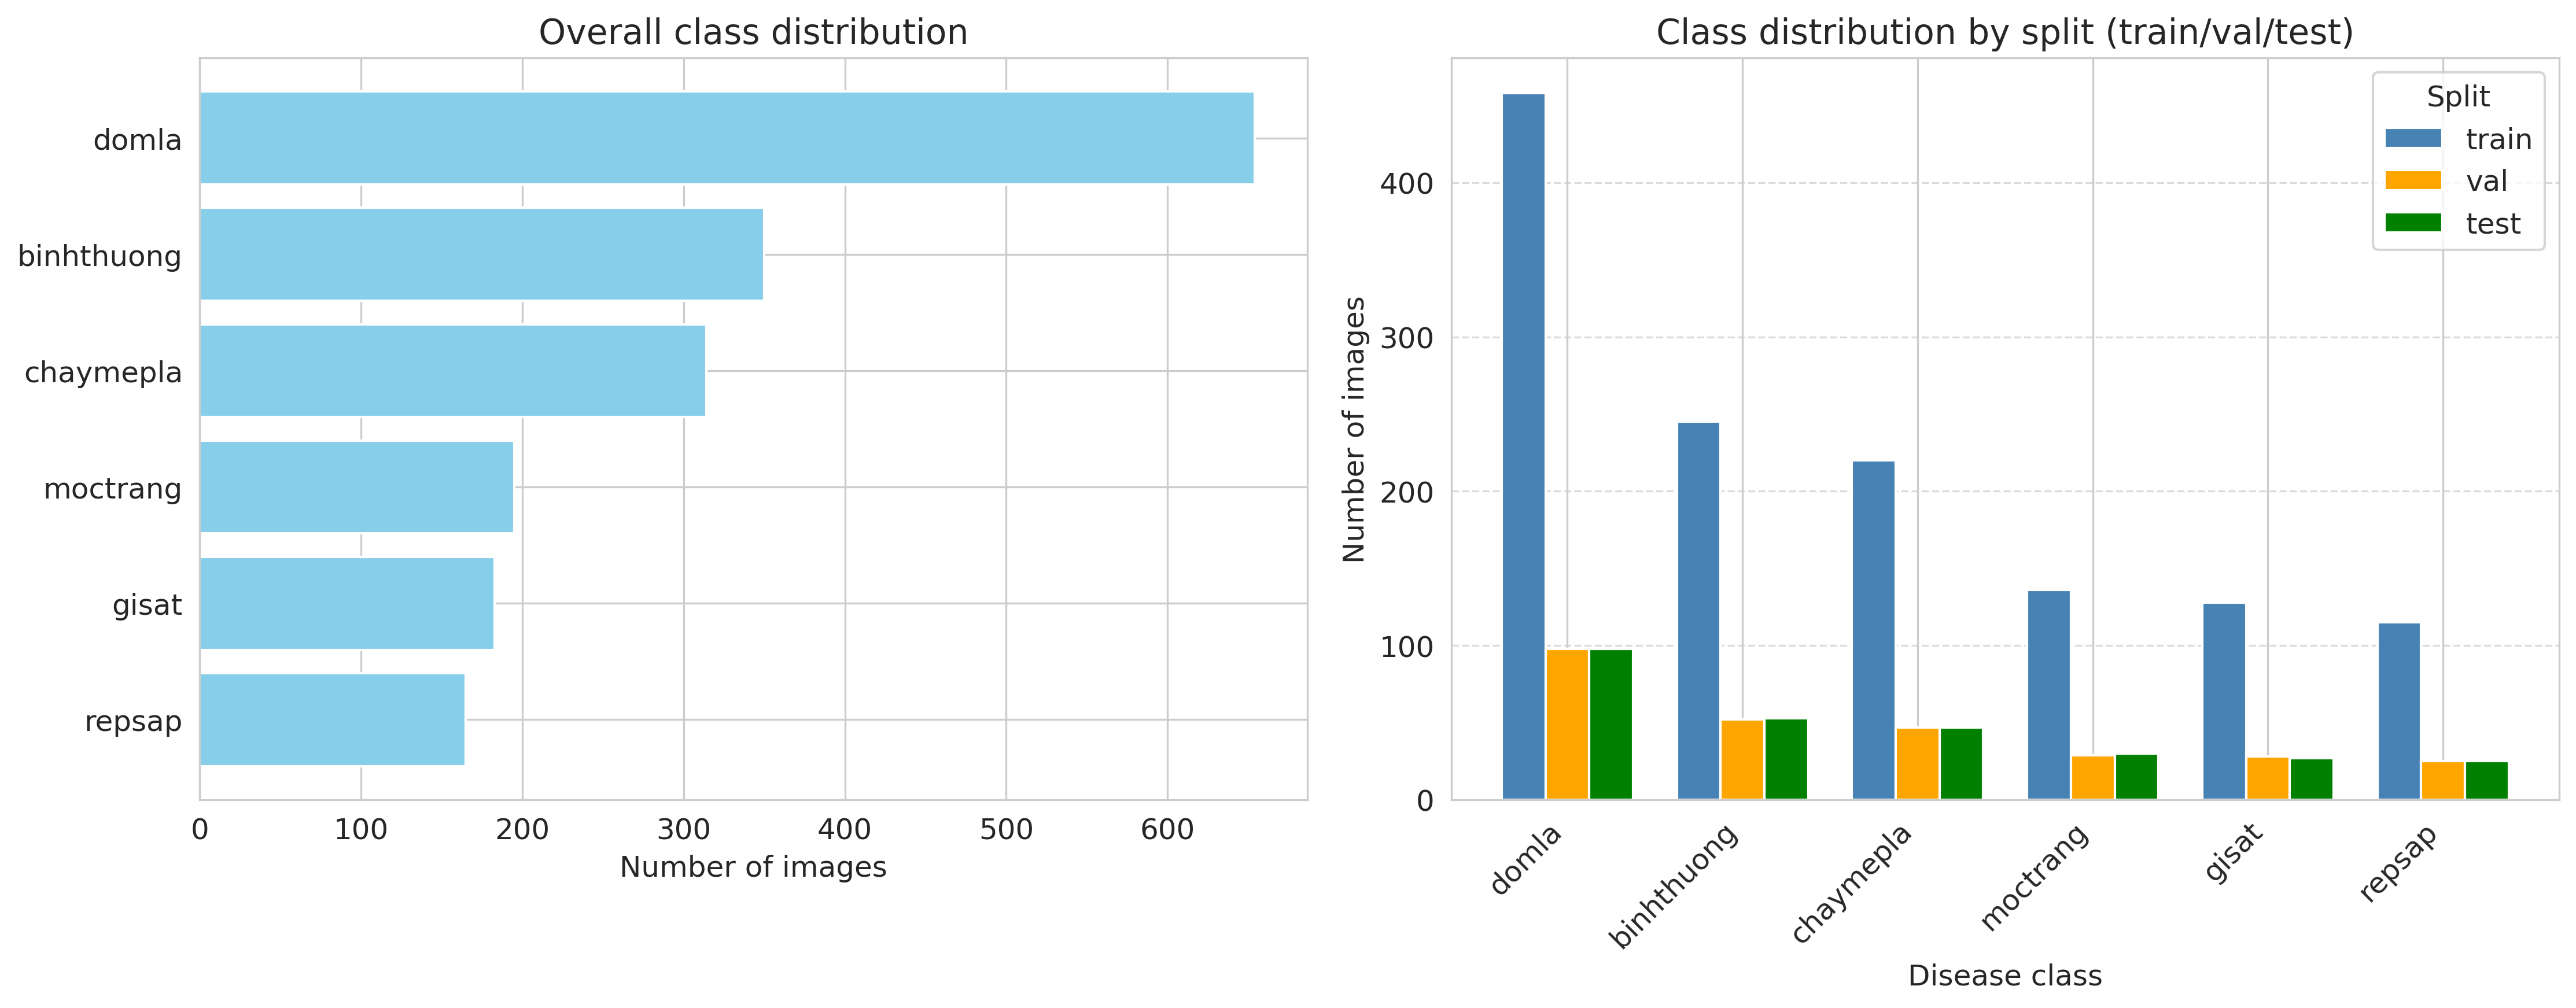
\includegraphics[width=\linewidth]{img/dataset/eda/class_distribution.png}
\caption{Class distribution. Left, overall bar chart. Right, grouped bar chart showing train/validation/test splits.}
\label{fig:class_dist}
\end{figure}


% =============================================
% Photometric Analysis
% =============================================
\subsection{Photometric Analysis}

As supporting evidence for the imaging diversity claimed in Section~\ref{sec:dataset_construction}, Figure~\ref{fig:brightness_contrast} shows that brightness varies substantially even within a single class (standard deviation 9.0 to 24.9 across classes), with \textit{domla} images alone spanning 44.4 to 153.9 and \textit{gisat} images spanning 80.5 to 182.1 on the 0-255 scale. Figure~\ref{fig:rgb_histograms} shows that classes also differ in dominant colour channel. These variations confirm that the images were collected under diverse, uncontrolled lighting and colour conditions rather than a single studio-like setup, and imply that models must be robust to such shifts rather than exploit them as shortcuts.

\begin{figure}[htbp]
\centering
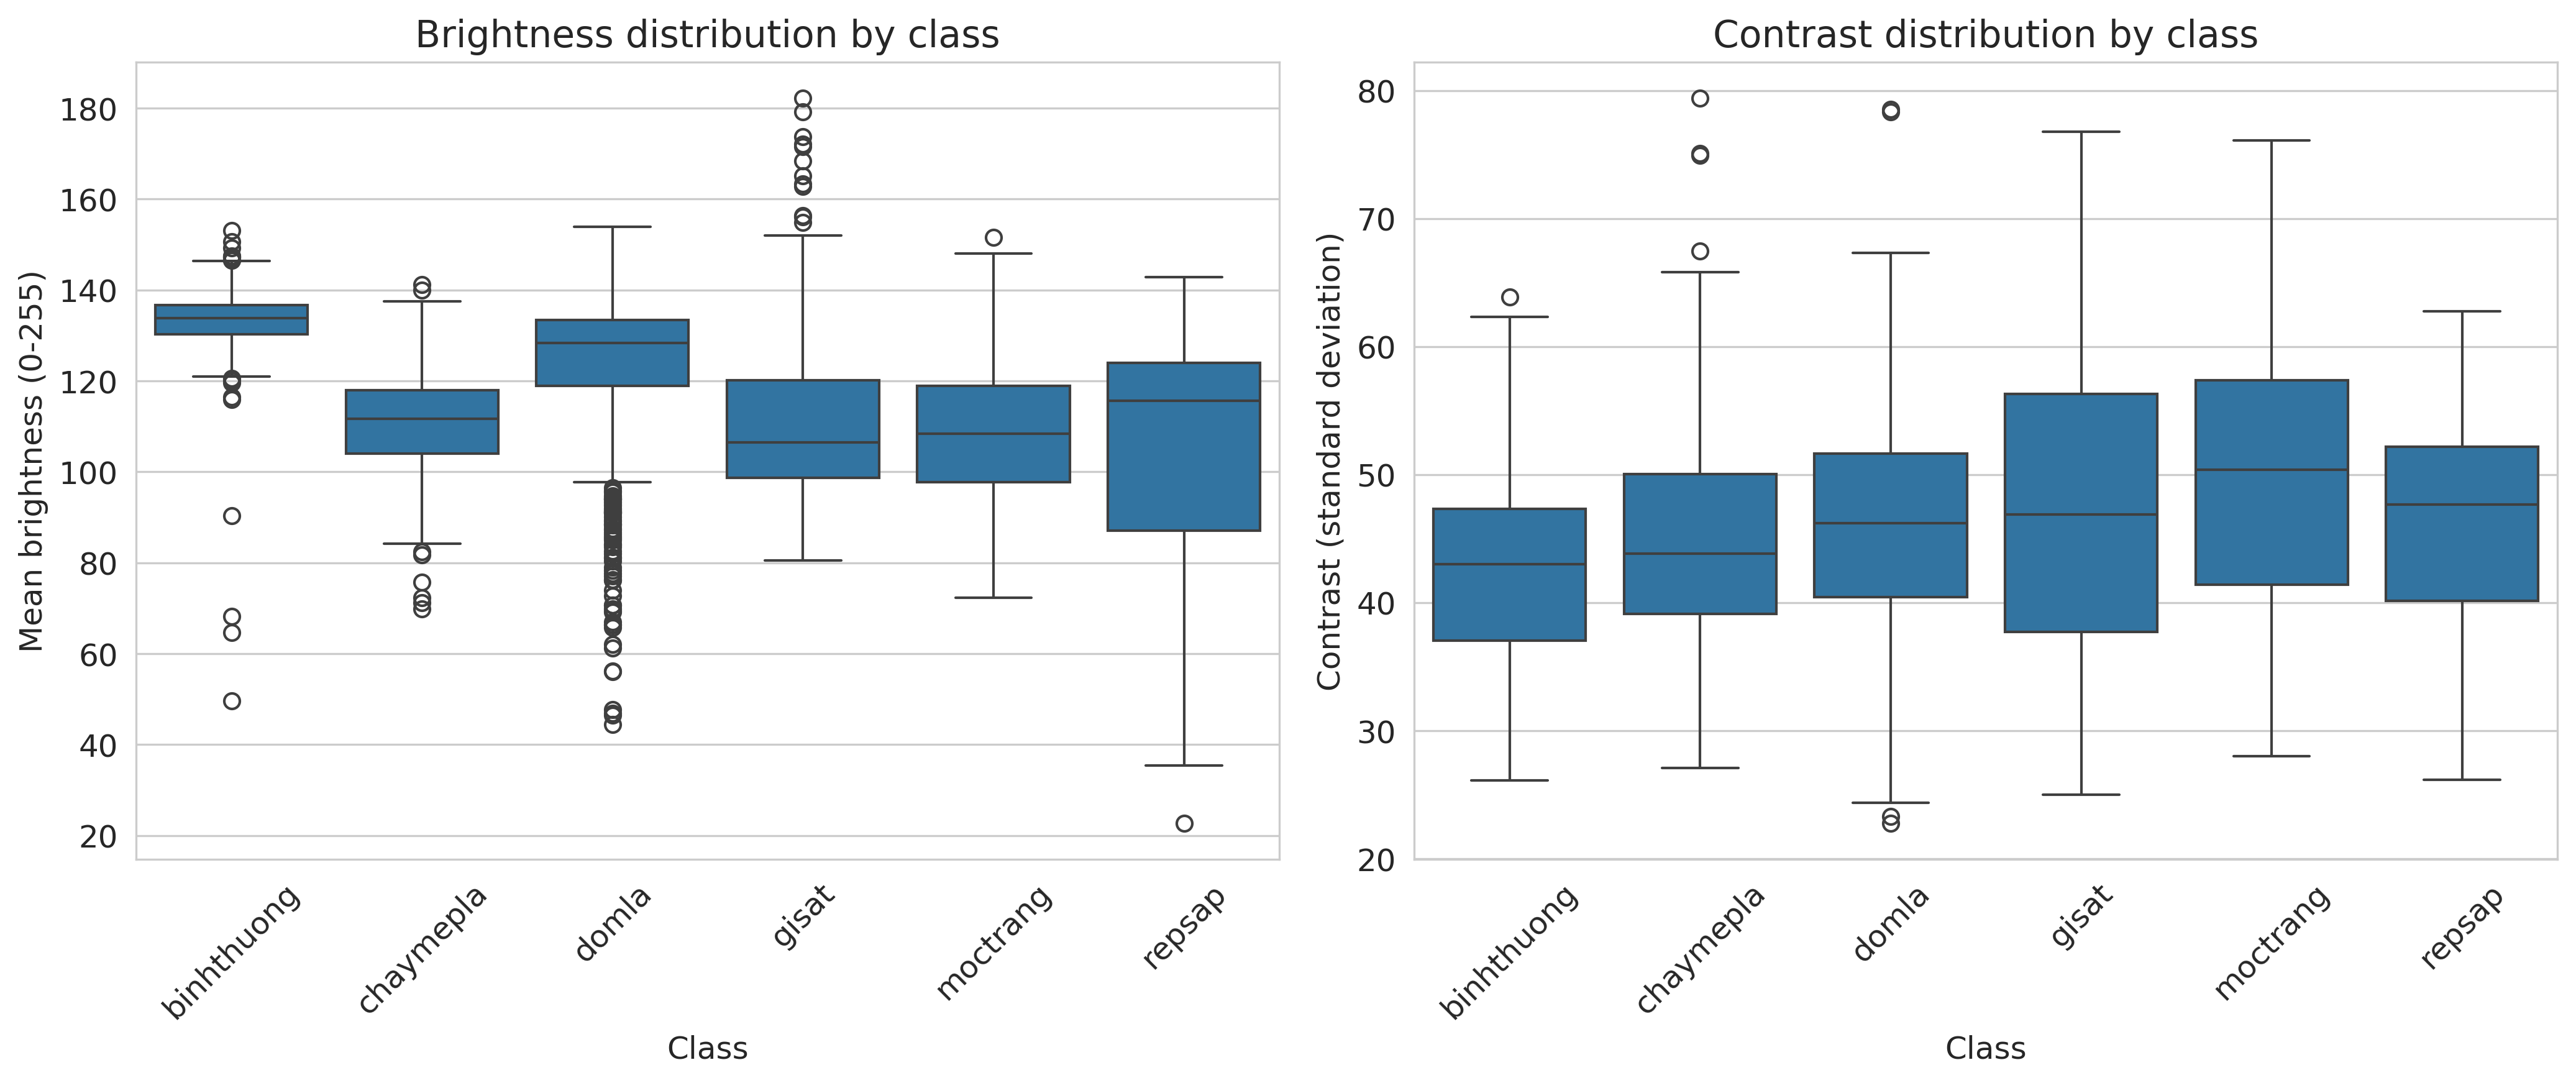
\includegraphics[width=\linewidth]{img/dataset/eda/brightness_contrast.png}
\caption{Brightness (left) and contrast (right) distributions per class.}
\label{fig:brightness_contrast}
\end{figure}

\begin{figure}[htbp]
\centering
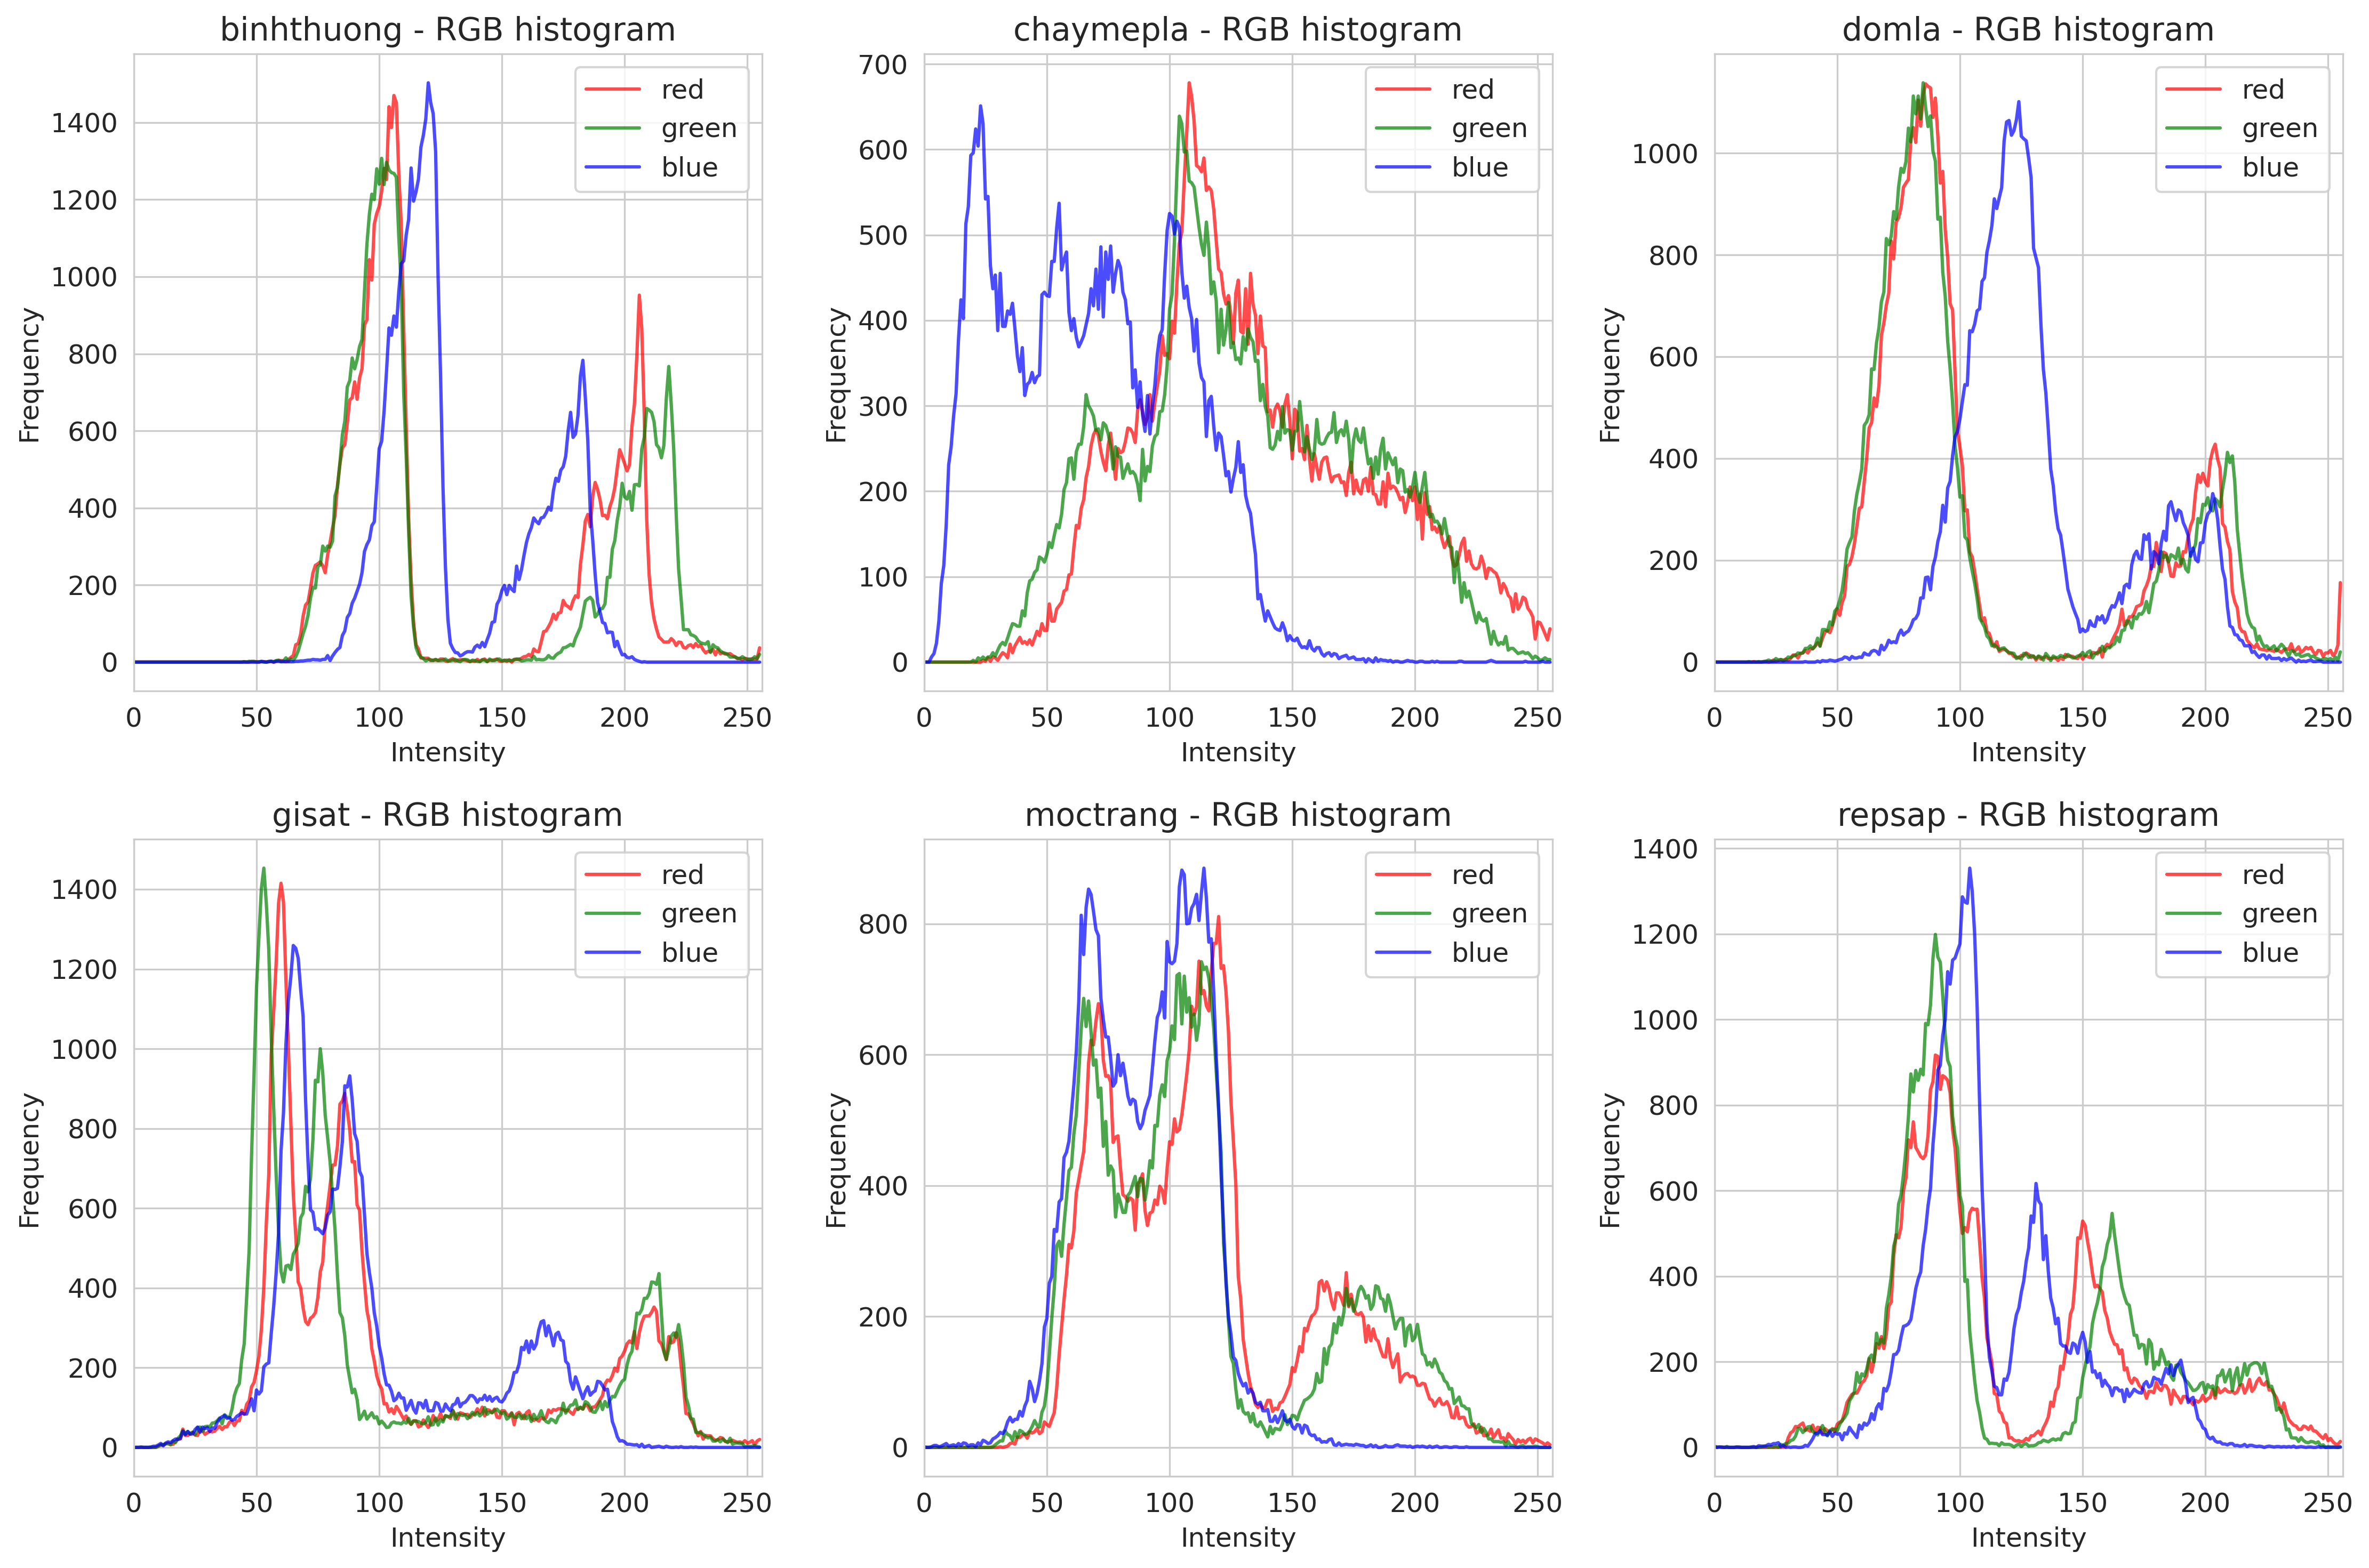
\includegraphics[width=\linewidth]{img/dataset/eda/rgb_histograms.png}
\caption{RGB histograms of one sample image per class (red, green, blue channels).}
\label{fig:rgb_histograms}
\end{figure}



% ===============================================
% Difficulty Analysis
% ===============================================
\subsection{Intrinsic Difficulty Analysis}
\label{subsec:difficulty}

To assess how challenging the dataset is for automatic classification, we performed three complementary analyses on the validation set using features extracted from a frozen ImageNet-pretrained ResNet-18 \citep{he2016deep}. The feature dimension was reduced to 512 via global average pooling.

\subsubsection{Quantitative Clustering Metrics}

We computed two standard metrics that evaluate class separability in the feature space, namely the Silhouette score \citep{rousseeuw1987silhouettes} and the Davies-Bouldin index \citep{davies1979cluster}. Table~\ref{tab:difficulty_metrics} summarises the results.

\begin{table}[htbp]
\centering
\caption{Quantitative difficulty metrics on the validation set. Lower Silhouette, higher Davies-Bouldin, and intra/inter ratio $\ge 1$ indicate strong class overlap.}
\label{tab:difficulty_metrics}
\begin{tabular}{l c}
\toprule
\textbf{Metric} & \textbf{Value} \\
\midrule
Silhouette Score & 0.0067 \\
Davies-Bouldin Index & 4.17 \\
Average intra-class distance & 12.82 \\
Average inter-class distance & 8.04 \\
Intra/Inter distance ratio & 1.59 \\
\bottomrule
\end{tabular}
\end{table}

The Silhouette score near zero indicates that samples are not closer to their own class than to neighbouring classes, implying heavy inter-class overlap. The Davies-Bouldin index (4.17) points in the same direction (lower is better separated, metric definition in \ref{app:difficulty}), though its absolute value is best read relative to other clustering configurations rather than against a fixed threshold, so it is reported here as a corroborating signal alongside Silhouette and the intra/inter distance ratio below. Notably, the intra/inter distance ratio exceeds 1 (1.59), meaning that within-class variation is larger than the separation between class centroids, a hallmark of fine-grained recognition problems.

\subsubsection{Visualisation with t-SNE}

\begin{figure}[H]
\centering
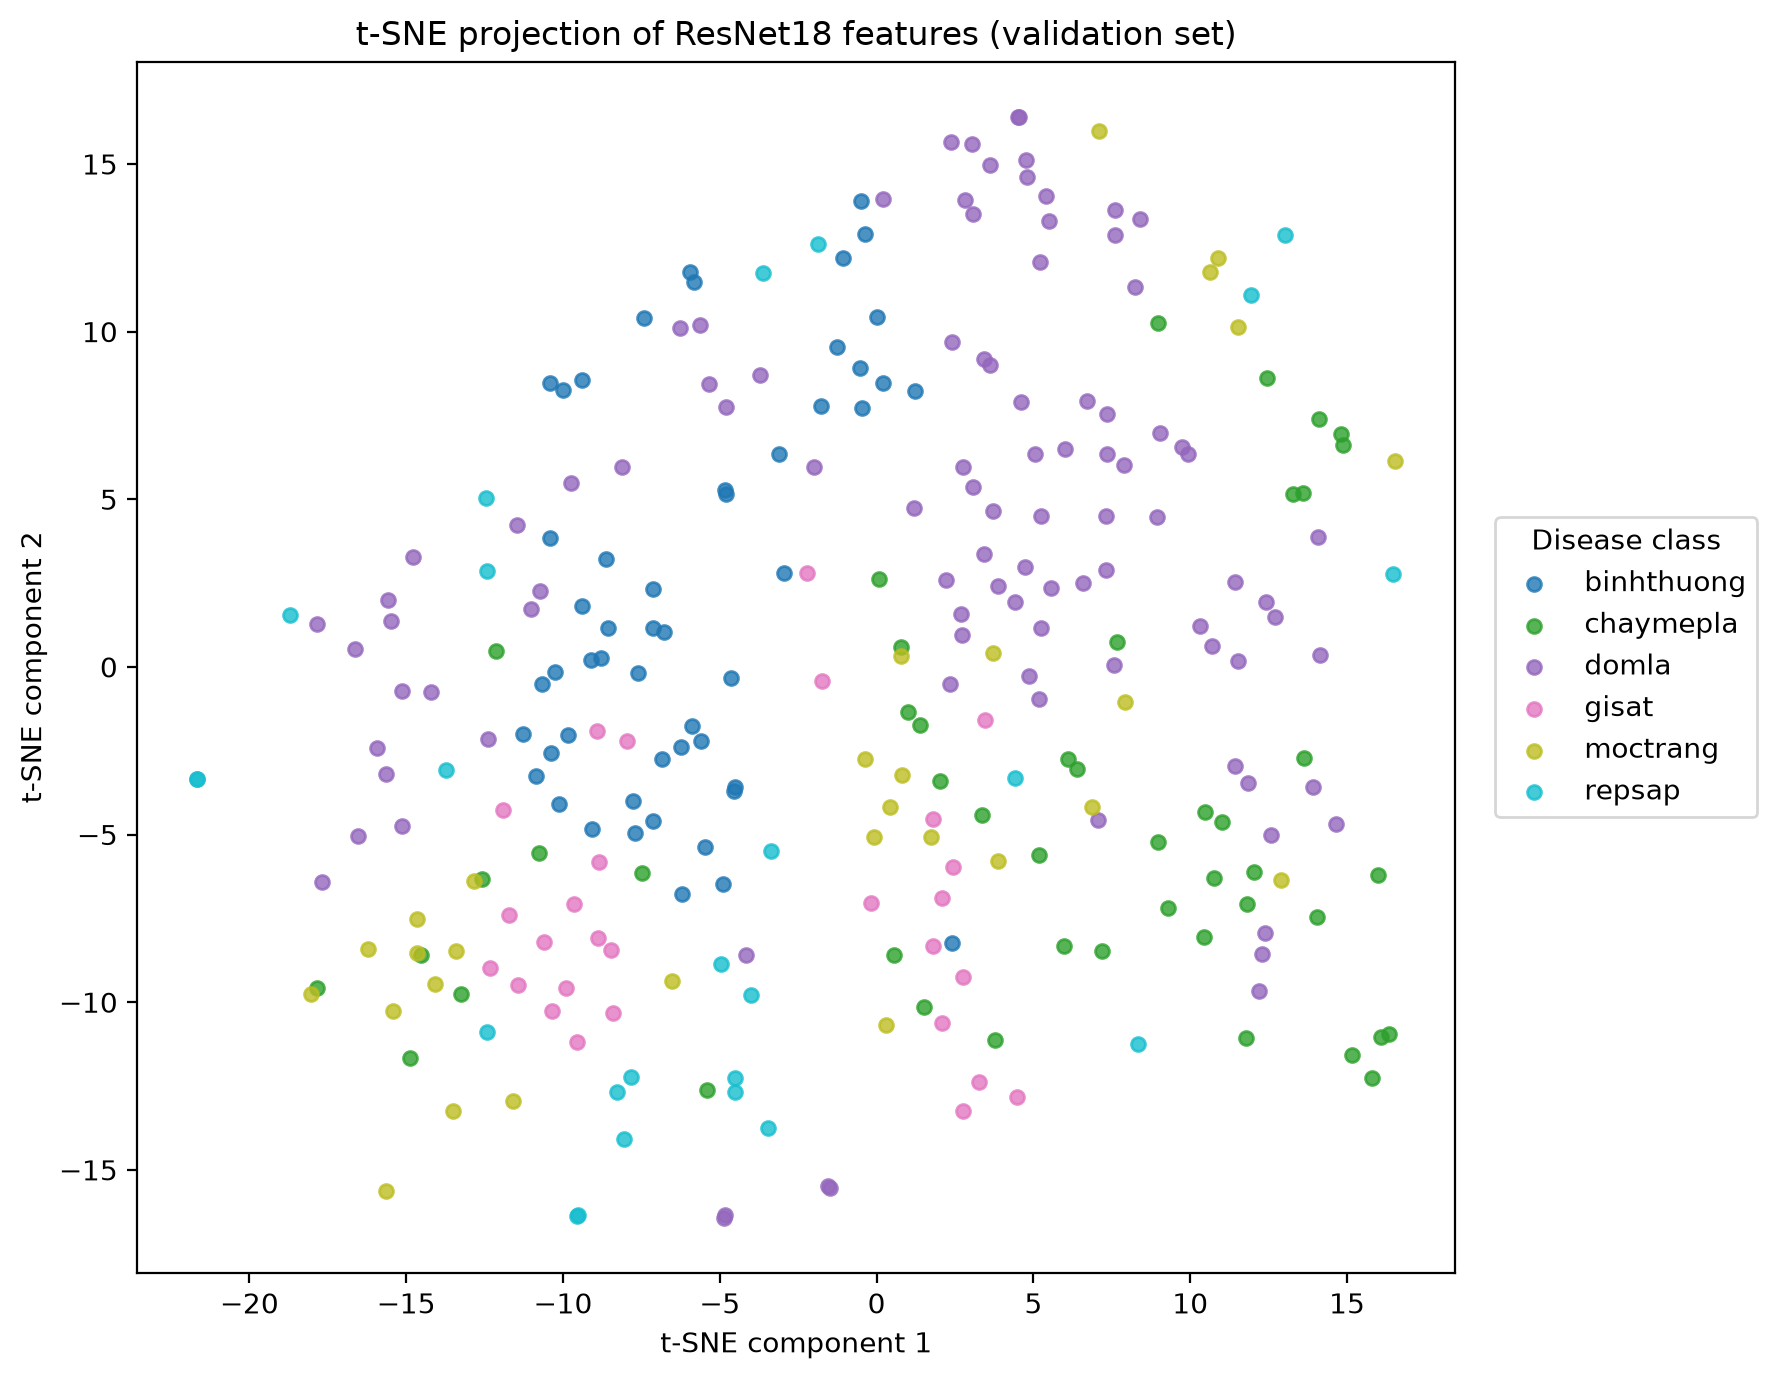
\includegraphics[width=0.8\columnwidth]{img/dataset/analysis/tsne_avocado_leaf.png}
\caption{t-SNE projection of ResNet-18 features on the validation set. Overlapping clusters confirm that disease categories are not well separated in the deep feature space.}
\label{fig:tsne}
\end{figure}

We projected the 512‑dimensional features into two dimensions using t-SNE \citep{maaten2008visualizing} with perplexity 30. Figure~\ref{fig:tsne} shows the resulting scatter plot, where each point represents a validation image and colours encode disease classes. All six classes exhibit substantial overlap without clear cluster boundaries. Classes with visually similar symptoms, such as \textit{chaymepla} (leaf scorch) and \textit{repsap} (mealybug damage), are heavily interleaved. This visual entanglement further confirms that the disease categories are not well separated in the deep feature space.

\subsubsection{Linear Separability Test}

To determine whether the frozen deep features are linearly separable by disease class, we trained a logistic regression classifier on the extracted features. Using 5‑fold cross‑validation, the model achieved a mean accuracy of \(75.25\% \pm 3.76\%\). When evaluated on a held‑out subset (30\% of the validation set, disjoint from the folds used above), the accuracy dropped to \(65.48\%\). Part of this gap is likely attributable to the small size of the validation set (279 images), which inflates the variance of both estimates. This attribution is qualitative. Unlike the architecture comparison in Section~\ref{sec:experiments} (\ref{app:bootstrap}), we did not compute a bootstrap confidence interval for the held-out estimate. The size of the reported drop should therefore be read as a point estimate whose own precision is not quantified here. Nonetheless, both figures are significantly better than random guessing (\(16.7\%\) for six classes). For comparison, Section~\ref{sec:experiments} shows that a fine-tuned, non-linear ConvNeXt-V2 model reaches \(92.14\%\) on this same AvocadoLeaf test set, a gap of roughly 17-27 percentage points over the linear probe depending on which estimate (\(75.25\%\) or \(65.48\%\)) is used. Hence, the disease classes are \textbf{not linearly separable} in the feature space, requiring non‑linear models or fine‑tuning to achieve satisfactory accuracy.

Taken together, the three analyses in this section are consistent with one another. Near-zero Silhouette, high Davies-Bouldin, and an intra/inter distance ratio above 1 all indicate substantial class overlap in feature space. The t-SNE visualisation shows this overlap directly. The linear probe confirms that this overlap cannot be resolved by a linear decision boundary. This motivates both the comparison of non-linear, fine-tuned architectures in Section~\ref{sec:experiments} and, more specifically, the use of metric-based few-shot learning in Section~\ref{subsec:fewshot}. Since frozen features are not linearly separable, a classifier trained directly on top of them generalises poorly, whereas prototypical networks learn a task-adapted embedding space in which the classes become separable.
% \section{Proposed Lightweight Model}
\label{sec:proposed_model}

Rather than designing a new architecture from scratch, we adopt a systematic \emph{selection-and-adaptation} approach. A broad pool of existing lightweight and efficient architectures is fine-tuned under a largely shared training protocol, with the deviations documented below, on the AvocadoLeaf dataset, and the best-performing candidate under joint accuracy-size-latency constraints is proposed as the deployment model for this task (Section~\ref{sec:experiments}). This section describes the candidate pool, the transfer-learning strategy applied to each, and the shared training protocol.

\subsection{Candidate Architectures}

We evaluate 15 architectures spanning five groups (a finer split of the three broader CNN / hybrid CNN-Transformer / pure-transformer families referenced in Section~\ref{sec:related_work}):
\begin{enumerate}
    \item[(1)] a Vanilla CNN trained from scratch as a minimal baseline.
    \item[(2)] a ResNet-18 \citep{he2016deep} baseline.
    \item[(3)] mobile-oriented CNNs (MobileNet-V2 \citep{sandler2018mobilenetv2}, MobileNet-V4 \citep{qin2024mobilenetv4}, TinyNet \citep{han2020tinynet}, GhostNet-V2 \citep{tang2022ghostnetv2}, EfficientNet-B0 \citep{tan2019efficientnet}).
    \item[(4)] hybrid CNN-Transformer designs (MobileOne \citep{vasu2023mobileone}, EdgeNeXt \citep{maaz2022edgenext}, FastViT \citep{vasu2023fastvit}, EfficientViT \citep{liu2023efficientvit}, ConvNeXt-V1 \citep{liu2022convnet}, ConvNeXt-V2 \citep{woo2023convnextv2}).
    \item[(5)] pure vision transformers (ViT-B/16 \citep{dosovitskiy2021vit}, SwinTransformer \citep{liu2021swin}).
\end{enumerate}
All architectures except Vanilla CNN are initialised from ImageNet-pretrained weights obtained from \texttt{torchvision} or \texttt{timm}.

\subsection{Transfer-Learning Strategy}

Because the AvocadoLeaf training set is comparatively small (1,302 training images across six classes), fully fine-tuning all layers of large pretrained backbones risks overfitting. We therefore apply \emph{selective layer unfreezing}. For every pretrained model, all backbone weights are frozen except the last one to two stages (or the last two encoder layers, for the transformer-based models) and a newly initialised classification head sized to the six AvocadoLeaf classes. Table~\ref{tab:finetune_strategy} summarises the unfreezing strategy per architecture family. The Vanilla CNN baseline has no pretrained weights and is instead trained end-to-end from random initialisation.

\begin{table*}[htbp]
\centering
\caption{Transfer-learning strategy by architecture family.}
\label{tab:finetune_strategy}
\small
\begin{tabularx}{\textwidth}{l X l}
\toprule
\textbf{Architecture family} & \textbf{Members} & \textbf{Unfrozen layers} \\
\midrule
Vanilla CNN & -- & All (trained from scratch) \\
ResNet-18 & -- & \texttt{layer4} + classifier head \\
Mobile CNNs & MobileNet-V2, MobileNet-V4, TinyNet, GhostNet-V2, EfficientNet-B0 & Last 2 feature blocks + head \\
Hybrid CNN-Transformer & MobileOne, EdgeNeXt, FastViT, EfficientViT, ConvNeXt-V1, ConvNeXt-V2 & Last 2 stages + head \\
Vision Transformers & ViT-B/16, SwinTransformer & Last 2 encoder layers + head \\
\bottomrule
\end{tabularx}
\end{table*}

\subsection{Training Protocol}

All 15 models share the same optimiser, learning-rate schedule, epoch budget, and data augmentation policy, using AdamW (learning rate $1\times10^{-4}$, weight decay $1\times10^{-4}$) with cosine-annealing decay over a maximum of 100 epochs, cross-entropy loss, and early stopping with a patience of 5 epochs on validation loss. Input images are resized to $224\times224$ and normalised using ImageNet statistics. Training-time data augmentation consists of random-resized cropping (scale $0.6$–$1.0$), horizontal flipping, random rotation ($\pm15^\circ$, applied with probability 0.3), colour jittering (brightness/contrast/saturation/hue), and random erasing. Models are always evaluated without augmentation at validation and test time.

Two aspects of this protocol are not held perfectly constant across all 15 candidates. First, the unfrozen-layer depth in Table~\ref{tab:finetune_strategy} differs between ResNet-18 (one stage) and the remaining pretrained models (two stages or encoder layers). Second, despite the augmentation policy above being intended uniformly, the ConvNeXt-V2/BoVien checkpoint reported in Section~\ref{sec:experiments} was in fact trained with augmentation disabled, and this switch was not applied consistently across all candidates. The ablation study (Section~\ref{subsec:ablation}) examines its effect on BoVien directly. See the Limitations discussion (Section~\ref{sec:discussion}) for further detail on both points.

The architecture that achieves the best joint accuracy-size-latency trade-off under this protocol, ConvNeXt-V2, is adopted as our proposed lightweight model for avocado disease classification. The full comparison against the other 14 candidates is reported in Section~\ref{sec:experiments}.

\subsection{Proposed Model Architecture}
\label{subsec:proposed_architecture}

As introduced in Section~\ref{sec:introduction}, we name the resulting deployment model \textbf{BoVien}, the \texttt{convnextv2\_atto} variant of ConvNeXt-V2 (3.7M parameters with its original 1000-way ImageNet head, 0.55 GFLOPs at $224\times224$), the smallest in the ConvNeXt-V2 family, adapted to AvocadoLeaf via the selective layer unfreezing strategy of Table~\ref{tab:finetune_strategy}. Replacing this head with the six-way AvocadoLeaf classification head used throughout this paper brings the parameter count down to the 3.4M reported in Table~\ref{tab:arch_compare}. Figure~\ref{fig:proposed_architecture} details its architecture. Box width encodes channel count, and box height/depth encode spatial resolution. Each stage's internals are grouped into a single box instead of listing every submodule. Reading left to right, a $4\times4$/stride-4 convolutional stem produces a $56\times56\times40$ feature map, which then passes through four stages of ConvNeXt-V2 blocks (depths 2-2-6-2, widths 40-80-160-320) with $2\times2$ downsampling between stages, ending at $7\times7\times320$. This is visible in the figure as boxes that shrink in height/depth (spatial resolution) while growing in length (channel count). Following Table~\ref{tab:finetune_strategy}, Stages~1-2 (grey) remain frozen at their ImageNet-pretrained weights, while Stages~3-4 (orange) are fine-tuned on AvocadoLeaf. Each stage is a stack of ConvNeXt-V2 blocks, each consisting of a $7\times7$ depthwise convolution, LayerNorm, an inverted-bottleneck MLP ($C\!\to\!4C\!\to\!C$) with GELU activation, and Global Response Normalisation (GRN) inserted between the two pointwise layers (the modification that distinguishes ConvNeXt-V2 from ConvNeXt-V1's LayerScale-based block), the whole block wrapped in a residual connection. The classification head (global average pool $\to$ LayerNorm $\to$ linear) is entirely new (green) and pools the $320$-d backbone feature, mapping it to a probability over the six AvocadoLeaf classes, kept deliberately narrow in the figure since it carries only 6 output channels. The leftmost image is a real (background-removed) AvocadoLeaf training sample, shown at its actual $224\times224\times3$ input resolution. In the remainder of the paper, ``ConvNeXt-V2'' refers to this candidate within the 15-architecture comparison (Section~\ref{sec:experiments}), and ``BoVien'' refers specifically to it once selected as the final proposed model.

\begin{figure*}[t]
\centering
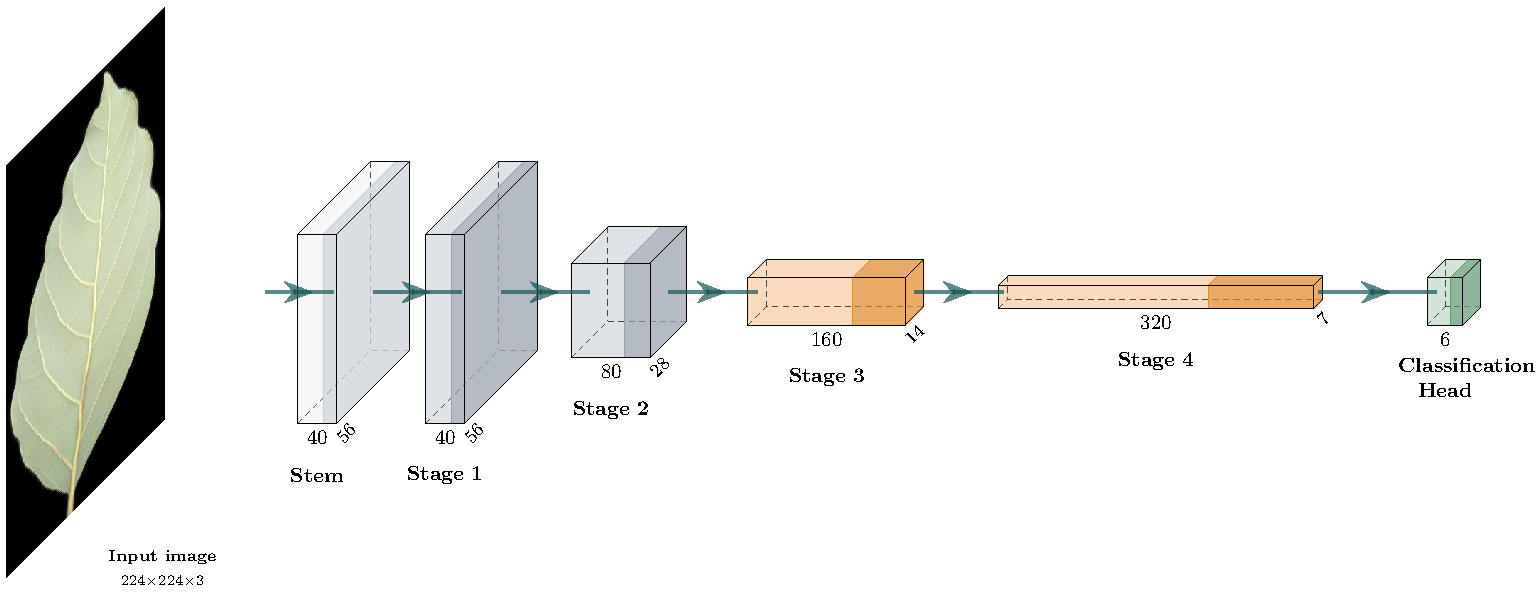
\includegraphics[width=0.75\textwidth]{img/models/proposed_architecture.pdf}
\caption{Architecture of Model BoVien. Grey indicates frozen (ImageNet-pretrained, unchanged) parameters, orange indicates parameters fine-tuned on AvocadoLeaf, and green indicates newly initialised, always-trainable parameters.}
\label{fig:proposed_architecture}
\end{figure*}

\section{Experiments and Results}
\label{sec:experiments}

\subsection{Comparison of Architectures}
\label{subsec:arch_compare}

We benchmark a wide range of lightweight and efficient architectures on the AvocadoLeaf test set. Table~\ref{tab:arch_compare} reports top-1 accuracy, macro F1 score, number of parameters, and per-image inference time on a single NVIDIA RTX 3050-6GB GPU for all 15 evaluated models. All models share the same optimiser, learning-rate schedule, and data augmentation policy (Section~\ref{sec:proposed_model}). Each architecture was trained once (single seed); to account for the uncertainty this and the finite 280-image test set introduce, we additionally report bootstrap 95\% confidence intervals and paired significance tests in \ref{app:bootstrap}.

\begin{table*}[t]
\centering
\caption{Performance comparison of all evaluated architectures. The highest values in each column are highlighted in bold and underlined.}
\label{tab:arch_compare}
\small
\setlength{\tabcolsep}{3pt}
\begin{tabularx}{\textwidth}{X c c c c}
\toprule
\textbf{Model} & \makecell[c]{\textbf{Acc}\\(\%)} & \makecell[c]{\textbf{Macro F1}} & \makecell[c]{\textbf{Params}\\(M)} & \makecell[c]{\textbf{Inference}\\(ms)} \\
\midrule
ConvNeXt-V2            & \textbf{\underline{92.14}} & 0.900 &  3.4 & 2.30 \\
SwinTransformer        & 91.43 & 0.899 & 27.5 & 6.69 \\
MobileOne              & 91.43 & 0.893 &  4.3 & 8.35 \\
ConvNeXt-V1            & 91.07 & 0.895 & 27.8 & 5.24 \\
ViT                    & 91.07 & \textbf{\underline{0.904}} & 85.8 & 14.25 \\
EdgeNeXt               & 91.07 & 0.877 &  5.3 & 3.75 \\
ResNet-18              & 88.93 & 0.863 & 11.2 & 1.98 \\
TinyNet                & 88.21 & 0.863 &  4.9 & 3.66 \\
FastViT                & 87.50 & 0.853 &  3.3 & 3.63 \\
MobileNet-V2           & 87.14 & 0.847 &  2.2 & 1.80 \\
EfficientNet-B0        & 86.43 & 0.838 &  4.0 & 2.85 \\
MobileNet-V4           & 76.07 & 0.724 &  2.5 & 1.89 \\
EfficientViT           & 69.29 & 0.650 &  3.2 & 7.00 \\
GhostNet-V2            & 69.29 & 0.571 &  4.9 & 5.43 \\
VanillaCNN             & 63.57 & 0.623 & 25.8 & 1.33 \\
\bottomrule
\end{tabularx}
\end{table*}


Among the evaluated models, ConvNeXt-V2 achieves the highest point-estimate classification accuracy (92.14\%) and the second-highest macro F1 score (0.900), while maintaining a compact parameter count (3.4M) and low inference latency (2.30 ms). However, bootstrap significance testing (\ref{app:bootstrap}) shows that its accuracy advantage over the next five models (SwinTransformer, MobileOne, ViT, EdgeNeXt, and ConvNeXt-V1) is \emph{not} statistically significant at this test set size ($p > 0.5$ for all five); these six models should be regarded as statistically tied in accuracy. In particular, ViT attains the highest macro F1 (0.904) but has 85.8M parameters and requires 14.25 ms per inference, making it impractical for edge deployment despite its statistically indistinguishable accuracy. What separates ConvNeXt-V2 from the rest of this tied top group is not proven superior accuracy but a far smaller parameter count (3.4M vs. 4.3--85.8M for the other five) and lower latency, which is why we select it as our proposed lightweight model. ConvNeXt-V2's advantage over every model ranked sixth or lower \emph{is} statistically significant ($p < 0.05$, \ref{app:bootstrap}). Conversely, lightweight architectures such as MobileNet-V2 and EfficientNet-B0 are faster and smaller but lag significantly in accuracy (approximately 86–87\%), which is insufficient for reliable field diagnosis. Models with accuracy below 80\% (MobileNet-V4, EfficientViT, GhostNet-V2, VanillaCNN) lack the representational capacity required for this fine-grained classification task. Overall, ConvNeXt-V2 offers the most favourable balance among accuracy, model size, and speed, making it the strongest candidate among the evaluated architectures for deployment on resource-constrained devices, pending on-device latency validation (Section~\ref{sec:discussion}).

To further understand the impact of model capacity, we group the 14 fine-tuned, ImageNet-pretrained architectures into two categories, including (1) \textit{lightweight models} with fewer than 5 million parameters (9 models) and (2) \textit{heavy models} with 5 million or more (5 models). The VanillaCNN baseline is excluded from this comparison: its 25.8M parameter count reflects an unoptimised from-scratch architecture rather than a deliberate heavy-model design choice, and including it by parameter count alone would place a 0.623 F1 score inside the heavy group purely as an artefact of training regime, not capacity. The heavy group achieves a high and stable mean F1 of 0.888, with all models scoring above 0.86. The light group shows much greater variance, with a mean of 0.793 and scores ranging from 0.571 to 0.900. 
ConvNeXt-V2 stands out as the only light model attaining F1 (0.900) comparable to the best heavy architectures while using substantially fewer parameters. This confirms that model selection is critical under parameter constraints, whereas heavy models offer stable performance at the cost of larger size and slower inference. 
\begin{figure}[htbp]
\centering
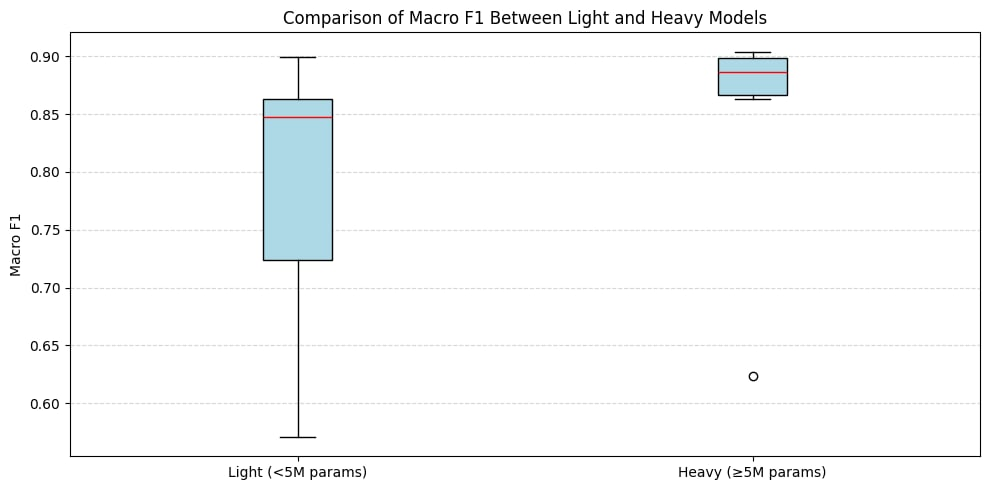
\includegraphics[width=\columnwidth]{img/models/f1_comparision.jpg}
\caption{Macro F1 scores of all evaluated models. Lightweight models (<5M parameters) are shown in blue, heavy models ($\geq$5M) in orange.}
\label{fig:f1_comparision}
\end{figure}


\subsubsection{Efficiency Analysis}
\label{subsec:efficiency}

To jointly assess accuracy, model size, and inference speed, we define a composite efficiency metric:

\[
\text{Efficiency} = \frac{\text{Macro F1}}{\text{Params (M)} \times \text{Inference Time (ms)}}.
\]

This metric quantifies the predictive performance achieved per unit of resource consumption, where higher values indicate better trade-offs among the three dimensions. Figure~\ref{fig:efficiency} visualises two complementary efficiency dimensions, F1 per million parameters (F1/Params) and F1 per millisecond inference time (F1/Time); the colour scale indicates macro F1.

\begin{figure}[htbp]
\centering
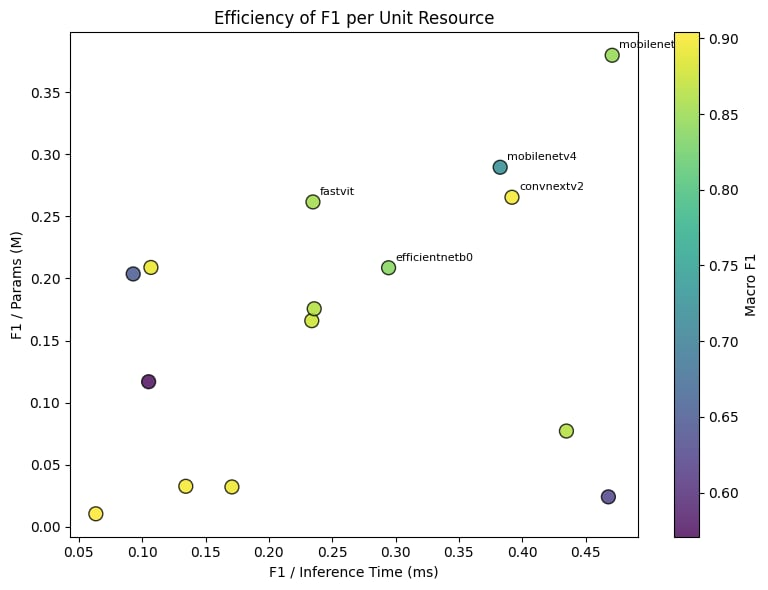
\includegraphics[width=\columnwidth]{img/models/efficiency.jpg}
\caption{Scatter plot of F1 per parameter versus F1 per inference time. Colour indicates macro F1.}
\label{fig:efficiency}
\end{figure}

MobileNet-V2 achieves the highest overall efficiency (0.211) due to its extremely compact size (2.2M parameters) and fast inference (1.80 ms), though its macro F1 (0.847) is moderate. ConvNeXt-V2 ranks third in efficiency (0.116) while attaining a substantially higher F1 (0.900). Its F1/Params (0.265) and F1/Time (0.391) are well balanced, placing it in the upper-right region of the scatter plot. Heavy models such as ViT (0.001) and SwinTransformer (0.005) exhibit very low efficiency despite competitive F1, due to large parameter counts and slower inference. These results indicate that ConvNeXt-V2 offers the most favourable balance between accuracy and resource utilisation among the evaluated architectures, based on parameter count and GPU inference latency.

\subsubsection{Ablation Study}
\label{subsec:ablation}

To isolate the contribution of two training-protocol switches exposed by our pipeline, namely data augmentation and class-weighted loss, we retrain Model BoVien (ConvNeXt-V2) under all four combinations, holding the architecture, optimiser, schedule, and epoch budget fixed. This does not repeat the full 15-architecture sweep; it only probes the proposed model itself. Each configuration is again trained once (single seed) on the same 280-image test set, so, following the same protocol as Section~\ref{subsec:arch_compare}, we report bootstrap 95\% confidence intervals and paired significance tests in \ref{app:bootstrap_ablation}.

\begin{table}[htbp]
\centering
\caption{Ablation of augmentation and class-weighted loss on Model BoVien (AvocadoLeaf test set).}
\label{tab:ablation}
\small
\begin{tabularx}{\columnwidth}{X c c}
\toprule
\textbf{Configuration} & \textbf{Acc (\%)} & \textbf{Macro F1} \\
\midrule
No augmentation, no class-weight   & \textbf{\underline{92.14}} & \textbf{\underline{0.900}} \\
No augmentation, class-weighted    & 90.71 & 0.887 \\
Augmentation, no class-weight      & 88.93 & 0.864 \\
Augmentation, class-weighted       & 91.43 & 0.895 \\
\bottomrule
\end{tabularx}
\end{table}

\begin{figure}[htbp]
\centering
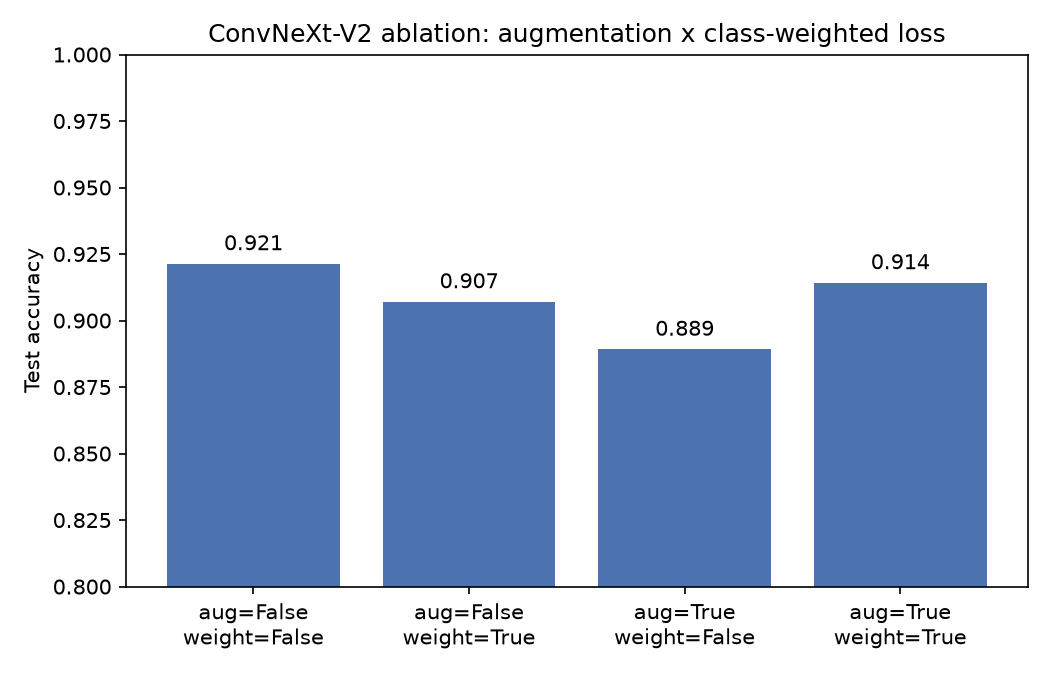
\includegraphics[width=\columnwidth]{img/experiments/ablation/ablation_accuracy.png}
\caption{Test accuracy of Model BoVien under the four augmentation $\times$ class-weighted-loss combinations.}
\label{fig:ablation}
\end{figure}

The no-augmentation, no-class-weight configuration is the best of the four, and its accuracy (92.14\%) matches the ConvNeXt-V2 row of Table~\ref{tab:arch_compare} exactly. This ablation grid includes the very checkpoint reported as our proposed model, not a separately retrained approximation of it, and confirms that the reported BoVien checkpoint was trained \emph{without} augmentation. This differs from the augmentation policy described in Section~\ref{sec:proposed_model}, which we flag as a documentation/protocol discrepancy in Section~\ref{sec:discussion} rather than silently reconcile here. Adding augmentation alone costs 3.2 accuracy points (92.14\% $\to$ 88.93\%), the largest single-factor drop in the grid, and adding class-weighting on top of augmentation recovers about two-thirds of that loss (88.93\% $\to$ 91.43\%) but still falls short of the no-augmentation baseline. Class-weighting alone also underperforms the plain baseline, though by a smaller margin (92.14\% $\to$ 90.71\%). A plausible explanation for augmentation hurting this particular model is that, on AvocadoLeaf's comparatively small training set (1,302 images), the added geometric and photometric perturbations remove information that ConvNeXt-V2's frozen-backbone-plus-fine-tuned-stages setup would otherwise use productively, though this ablation grid alone cannot rule out that the same holds for the other 14 candidate architectures. However, bootstrap significance testing (\ref{app:bootstrap_ablation}) shows that none of these three differences are statistically significant at this test set size, including the largest one (no augmentation, no class-weight, versus augmentation, no class-weight, $+$3.31pp, $p = 0.054$); the ranking above should therefore be read as suggestive rather than conclusive, consistent with how Section~\ref{subsec:arch_compare}'s single-seed, 280-image comparisons are treated throughout this paper.

\subsubsection{Error Analysis}
\label{subsec:error_analysis}

To characterise \emph{which} classes drive the remaining test-set errors, rather than only the aggregate 92.14\% figure, we re-examine BoVien's 280 per-image test predictions (already saved by the evaluation pipeline; no re-inference) through its confusion matrix.

\begin{figure}[htbp]
\centering
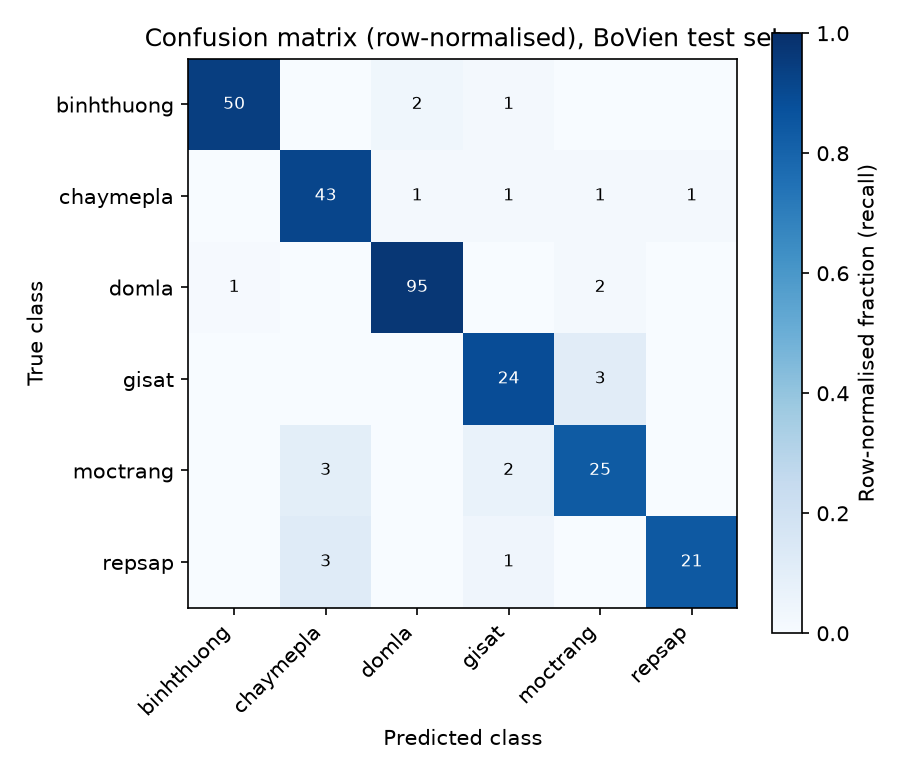
\includegraphics[width=\columnwidth]{img/experiments/evaluating/confusion_matrix_heatmap.png}
\caption{Row-normalised confusion matrix (raw counts annotated) for Model BoVien on the AvocadoLeaf test set.}
\label{fig:confusion_matrix}
\end{figure}

Per-class recall ranges from 96.9\% (\textit{domla}, the largest class at 458 training images) down to 83.3--84.0\% for the three smallest classes, \textit{moctrang} (136 training images, 83.3\% recall), \textit{repsap} (115, 84.0\%), and \textit{gisat} (128, 88.9\%), while the three larger classes (\textit{domla} 458, \textit{binhthuong} 245, \textit{chaymepla} 220) all exceed 91\% recall. This is consistent with a straightforward sample-size effect rather than any one class being intrinsically harder to photograph or define. The confusions are concentrated in three symmetric pairs: \textit{gisat} (algal leaf spot, orange velvety pustules) $\leftrightarrow$ \textit{moctrang} (powdery mildew, white powdery coating) account for 5 of 280 errors in both directions, \textit{repsap} (mealybug damage, silver/stippled marks) is confused with \textit{chaymepla} (leaf scorch, margin/tip burn) in 12.0\% of \textit{repsap} images, and \textit{moctrang} is likewise confused with \textit{chaymepla} in 10.0\% of its images. All three pairs share a plausible visual explanation: each involves a diffuse or patchy discolouration (algal spots, powdery coating, insect stippling) that can visually resemble scorch damage or a different spot pattern under variable field lighting, rather than the compact, high-contrast lesions of \textit{domla}. Notably, \textit{repsap} is also the class with the lowest LIME faithfulness score (Section~\ref{subsec:interpretability}, mean confidence drop 0.416 vs.\ 0.649 overall), so its diffuse, non-contiguous damage pattern appears to make it both harder to classify correctly and harder to explain with a fixed-size superpixel mask, two independent pieces of evidence pointing at the same underlying cause. Full per-class and per-pair breakdowns are in \texttt{deliverables/evaluating/\{per\_class\_error\_summary,confused\_pairs\}.csv}.

\subsection{Model Interpretability}
\label{subsec:interpretability}

To assess whether ConvNeXt‑V2 relies on disease‑relevant visual evidence rather than spurious correlations, we apply LIME \cite{ribeiro2016why} to every image in the 280-image test set (not merely a qualitative sample). Each image is segmented into superpixels with the Quickshift algorithm, and 500 perturbed samples are used to fit a local surrogate model that identifies the superpixels most responsible for the predicted class.

We quantify faithfulness with a deletion metric. For each test image, we hide exactly the superpixels LIME identifies as most responsible for the predicted class (the same masking colour used during LIME's own perturbation sampling) and re-run the model, measuring how much its confidence in the predicted class drops. A faithful explanation should cause a large drop, since it claims the hidden region is what the prediction relies on. Averaged over all 280 test images, hiding the LIME-highlighted region (which covers only 20.0\% of the image area on average) drops the model's confidence in its own predicted class from 0.940 to 0.292, a mean confidence drop of 0.649 (bootstrap 95\% CI [0.618, 0.678], see \ref{app:lime_faithfulness} for the full methodology and per-class breakdown). The drop is larger for correctly classified images (0.660, $n=258$) than for misclassified ones (0.516, $n=22$), consistent with correct predictions being more strongly grounded in genuine symptomatic regions rather than spurious cues. This full-test-set quantitative result substantially strengthens the qualitative examples below.

Figure~\ref{fig:lime_examples} shows two representative qualitative examples. For \textit{chaymepla}, the highlighted superpixels tightly enclose the brown, scorched lesion at the centre of the leaf, closely matching the visible symptom boundary. For \textit{moctrang} (powdery mildew), the highlighted regions concentrate on the white powdery patches on the leaf surface rather than on the unaffected tissue or background. These qualitative results illustrate that ConvNeXt‑V2's predictions are driven by the same visual cues a human expert would use, rather than by background or imaging artefacts, consistent with the quantitative deletion-metric result above.

\begin{figure}[htbp]
\centering
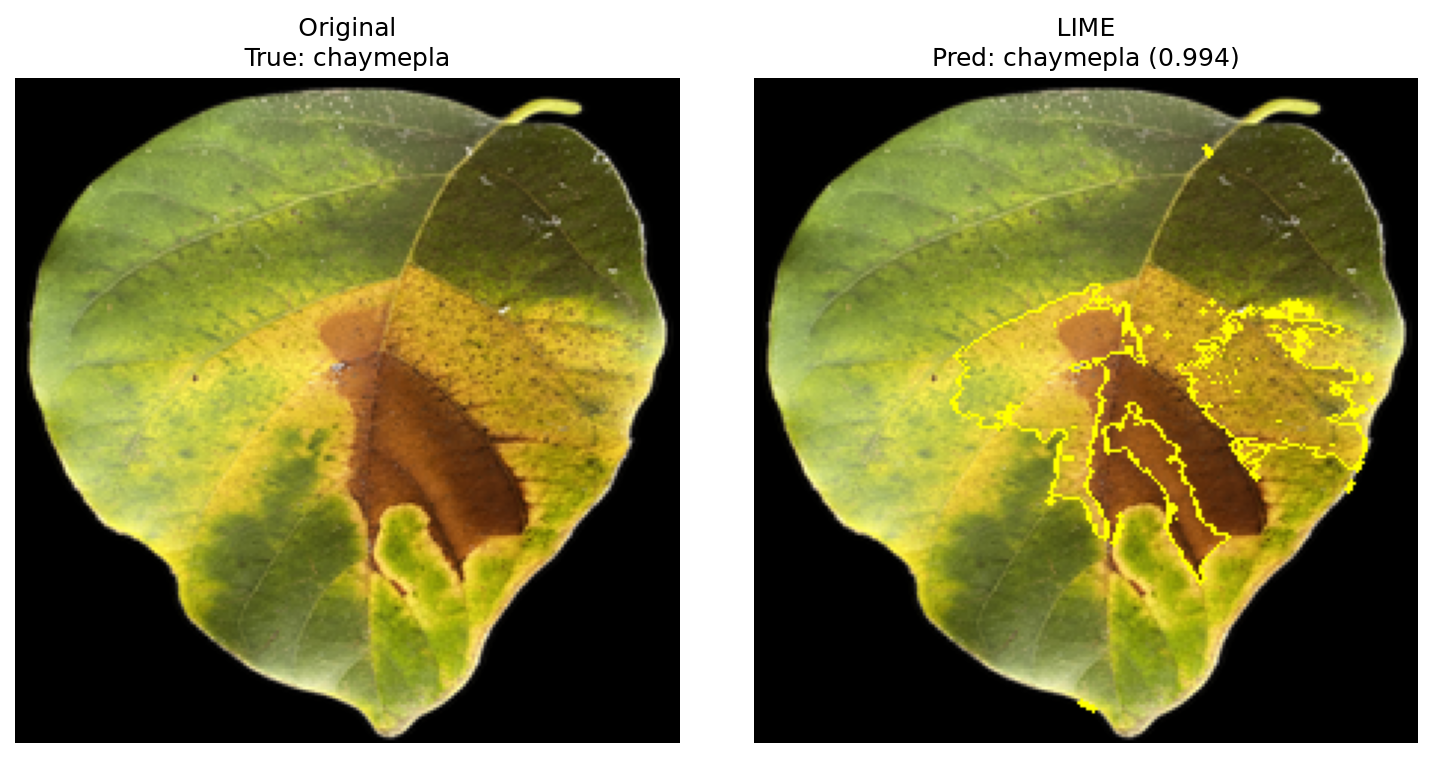
\includegraphics[width=0.49\linewidth]{img/experiments/xai/chaymepla_lime.png}
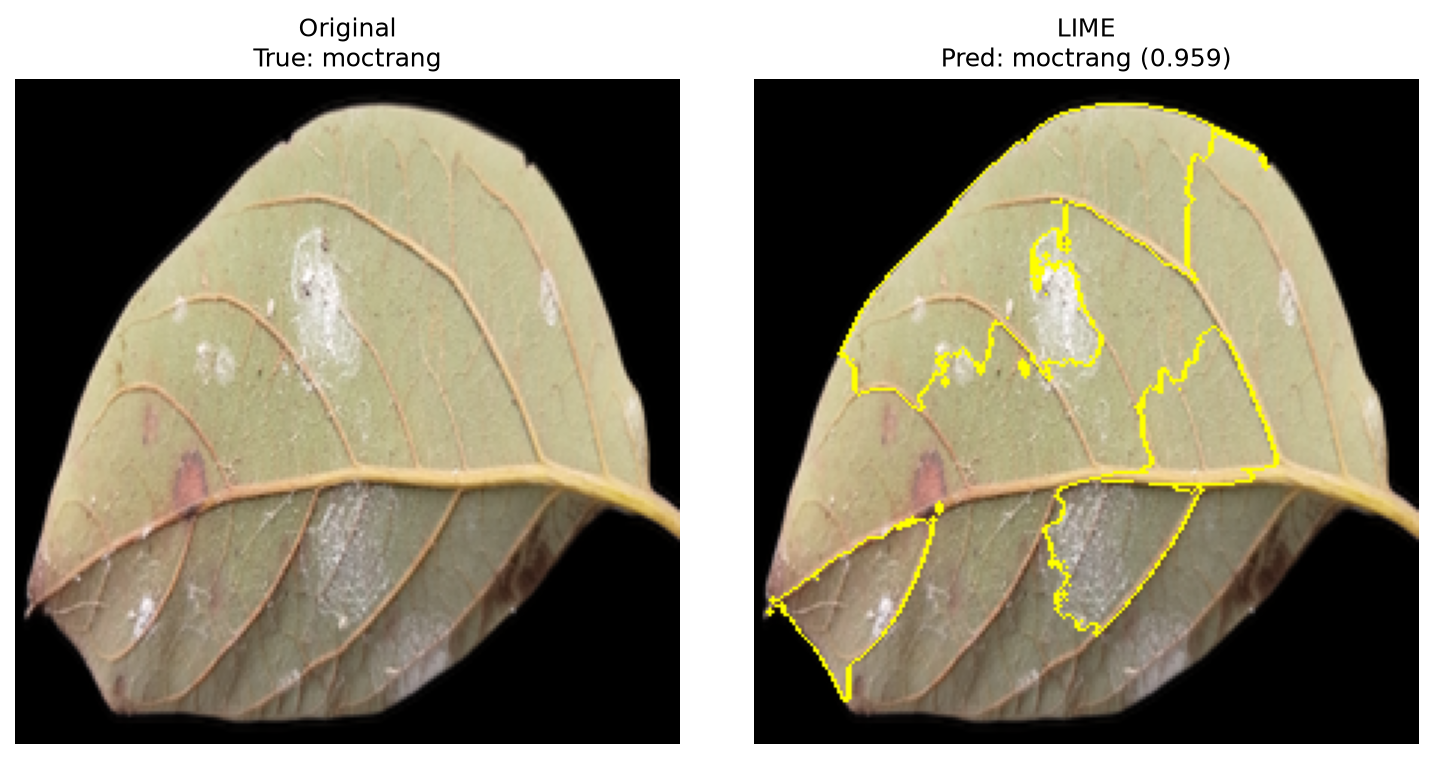
\includegraphics[width=0.49\linewidth]{img/experiments/xai/moctrang_lime.png}
\caption{LIME explanations for ConvNeXt‑V2 on two disease classes. Left, \textit{chaymepla} (leaf scorch), where the highlighted region matches the scorched lesion; right, \textit{moctrang} (powdery mildew), where the highlighted region matches the white powdery patches. Yellow outlines mark superpixels positively attributed to the predicted class.}
\label{fig:lime_examples}
\end{figure}

\subsection{Multi-modal Explanation Generation (CNN + LIME + VLM)}
\label{subsec:vlm_explain}

LIME identifies \emph{which pixels} a prediction depends on but produces no natural-language account of \emph{why} those pixels are diagnostically relevant, a gap that matters for a farmer-facing tool, where a highlighted region without a caption is of limited practical use. We therefore built a pipeline combining all three components developed in this work (the CNN's prediction, LIME's visual attribution, and a small, locally-hosted vision-language model, \texttt{Qwen2-VL-2B-Instruct}, no API cost) to generate a grounded natural-language explanation. Critically, the CNN remains the sole decision-maker. The VLM is given the CNN's already-decided class label together with the raw leaf image and the LIME overlay image, and is asked only to describe the visual evidence and judge whether it supports that label, never to propose a different one (\texttt{final\_pred} is verified to equal the CNN's prediction for 100\% of processed images). This design was applied to the 140 test images ConvNeXt‑V2 was least confident about (top 50\% by MC-Dropout predictive entropy).

Figure~\ref{fig:explain_vlm_showcase} shows three outputs of this pipeline, hand-selected from the 140-image escalated subset as coherent, correctly-grounded examples rather than a random or representative sample (full text in Table~\ref{tab:explain_vlm_showcase}). In these examples, the generated text correctly references both the LIME-highlighted location (e.g. ``vùng giữa hai lá'') and the specific visual symptom expected for the class (e.g. rust-coloured spots for \textit{gisat}, white powdery patches for \textit{moctrang}), demonstrating that the pipeline \emph{can} turn a raw prediction and an attribution map into an interpretable, farmer-readable statement, which was the original motivation for adding a language model to this system. Not every generated explanation is this coherent, however; Section~\ref{sec:discussion} discusses a case where the model's reasoning conflated the symptom description of a different class.

Across the full 140-image escalated subset, the VLM judged the visual evidence to support the CNN's diagnosis for 92.0\% of the 125 images that produced a parseable response. This figure should not be read as a validated accuracy or quality score; it is simply how often the model answered ``yes'', and it is in fact somewhat higher than ConvNeXt‑V2's own 85.0\% accuracy on this same subset (\ref{app:llm}). This is consistent with the low recall (0.21) for detecting actual mistakes reported in Section~\ref{sec:discussion}, as the model agrees with the CNN more often than the CNN is actually correct, suggesting a degree of acquiescence bias rather than critical evaluation of the evidence.

\begin{figure}[htbp]
\centering
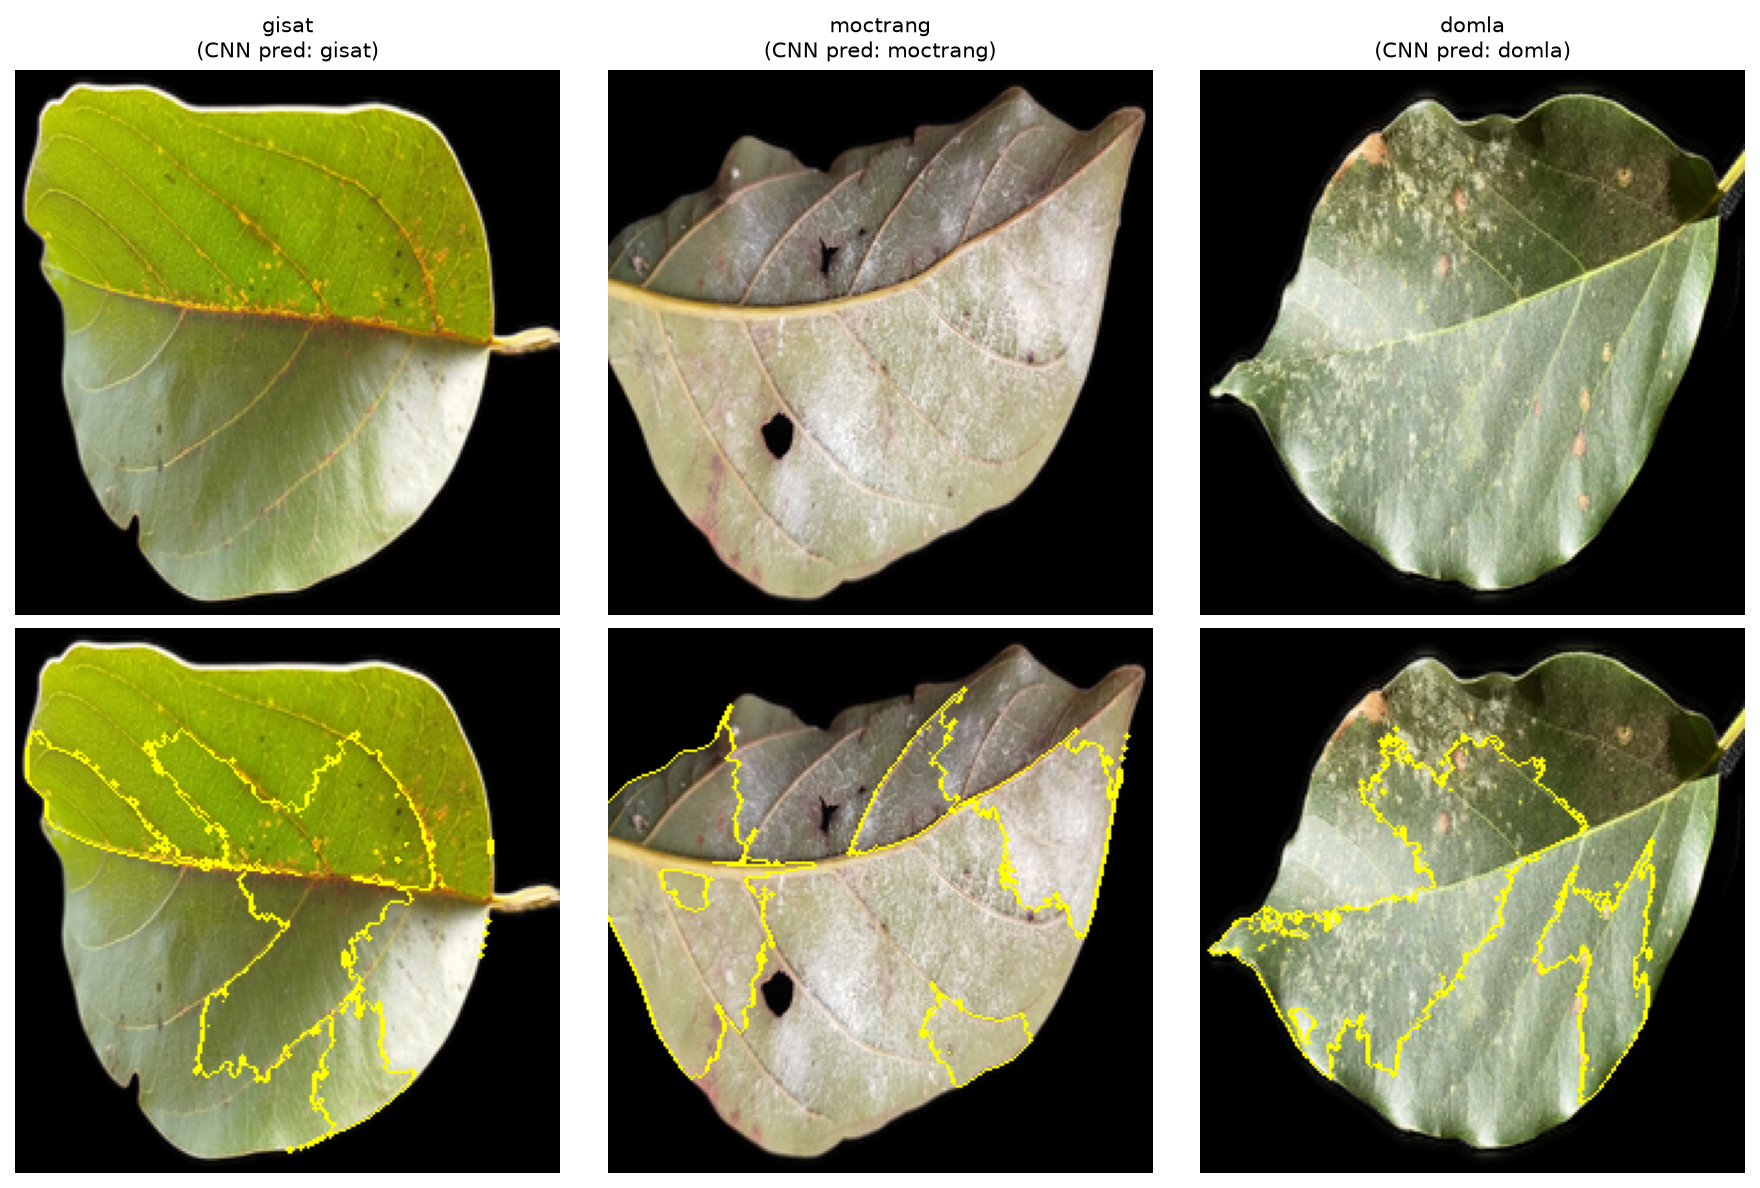
\includegraphics[width=\linewidth]{img/experiments/llm/explain_vlm_showcase.png}
\caption{Three examples of the combined CNN + LIME + VLM explanation pipeline. Top row, original test images; bottom row, LIME overlay (yellow outlines) shown to the VLM alongside the CNN's prediction. Generated explanations are given in Table~\ref{tab:explain_vlm_showcase}.}
\label{fig:explain_vlm_showcase}
\end{figure}

\begin{table}[htbp]
\centering
\caption{VLM-generated explanations for the three examples in Figure~\ref{fig:explain_vlm_showcase}, translated from Vietnamese.}
\label{tab:explain_vlm_showcase}
\small
\begin{tabular}{p{0.12\linewidth} p{0.78\linewidth}}
\toprule
\textbf{Class} & \textbf{Generated visual evidence} \\
\midrule
gisat & ``The CNN's most-attended region is in the middle of the leaf, particularly the area with rust-orange-coloured spots, typically on the underside -- this may be a sign of \textit{gisat}.'' \\
moctrang & ``The estimated region between the two images has many yellow-outlined patches, indicating white powdery spots on the leaf -- the CNN attended most to this region when predicting \textit{moctrang}.'' \\
domla & ``The CNN's most-attended region is near the centre of the leaf, close to the leaf-spot location; the spot's colour and shape resemble the small, round or irregular spots on the leaf surface [that define \textit{domla}].'' \\
\bottomrule
\end{tabular}
\end{table}

This capability is distinct from, and should not be conflated with, using the same VLM output as an automatic error detector. Section~\ref{sec:discussion} and \ref{app:llm} report a separate, secondary analysis of whether the \texttt{supports\_cnn\_diagnosis} judgement can substitute for or complement predictive-entropy-based flagging of likely CNN mistakes, which was \emph{not} successful. The explanation-generation capability demonstrated here is unaffected by that negative result; the pipeline is \emph{capable} of producing a plausible, grounded caption for a prediction, as shown by the curated examples above, though we have not established how often it does so unprompted across the full subset, nor validated the captions against expert judgement rather than an automated proxy. Whether such captions are a reliable enough signal to automatically flag errors without human review is a separate, harder question that Section~\ref{sec:discussion} answers in the negative for this specific use.


\subsection{Few-shot Learning}
\label{subsec:fewshot}

To evaluate the ability of our model to generalise from very few labelled examples – a realistic scenario in agricultural applications where data collection is expensive – we conducted few-shot experiments on the AvocadoLeaf dataset. We compared three approaches, namely (i) standard fine-tuning of the entire classifier on the limited support set (denoted as \texttt{Fine‑tune}), (ii) Prototypical Networks (ProtoNet) using a frozen ConvNeXt‑V2 backbone, and (iii) Relation Networks (RelationNet) with the same frozen backbone.

For each setting, we randomly sampled \(K\) images per class (\(K \in \{1,5,10,20\}\)) from the training set to form the support set, and evaluated on the full test set. Fine‑tune was trained for 50 epochs with early stopping; for ProtoNet and RelationNet we report the mean accuracy and standard deviation over 600 randomly generated episodes (6‑way, \(K\)-shot, 5 query images per class).

The quantitative results are summarised in Table~\ref{tab:fewshot_results}, and a visual comparison is provided in Figure~\ref{fig:fewshot_acc}. Several observations can be made:

\begin{itemize}
    \item \textbf{Fine‑tune suffers from severe overfitting} when only a few samples per class are available. With only 5 shots, it achieves only 16.4\% accuracy, and even with 20 shots it reaches only 28.6\%, indicating that conventional fine‑tuning is not suitable for extreme low‑data regimes.
    
    \item \textbf{Prototypical Networks substantially outperforms fine‑tuning at all shot levels.} Already with 1 shot per class, ProtoNet attains 28.9\% accuracy, which is higher than fine‑tuning with 5 shots (16.4\%). The gap remains large as the number of shots increases. At 5 shots ProtoNet achieves 45.7\% (+29.2 p.p.), at 10 shots 52.3\% (+31.3 p.p.), and at 20 shots 57.4\% (+28.9 p.p.). These results demonstrate that metric‑based few‑shot learning is substantially more effective than fine‑tuning for fine‑grained plant disease classification, even though absolute accuracy remains moderate.
    
    \item \textbf{Relation Networks perform poorly} on this dataset, with accuracy remaining close to the 16.7\% random-chance baseline (16–19\%) across all shot levels and showing no consistent improvement as the number of shots increases (see Figure~\ref{fig:fewshot_acc}). This suggests that the learnable distance metric of RelationNet may overfit to the specific episode composition or that the relation module requires more training data to generalise.
\end{itemize}

Overall, the ProtoNet framework combined with a frozen ConvNeXt‑V2 backbone provides the strongest few‑shot baseline among the three methods evaluated, more than doubling fine‑tuning's accuracy at every shot level tested and reaching 57.4\% accuracy with only 20 labeled images per class. While this is well below the $>$90\% accuracy achieved with the full training set (Table~\ref{tab:arch_compare}), it demonstrates that metric-based few-shot learning is a substantially more data-efficient starting point than fine-tuning for scenarios where data collection is expensive.

\begin{table*}[t]
\centering
\caption{Few-shot classification accuracy (\%) on the test set. Fine‑tune results are from a single training run; ProtoNet and RelationNet results are averaged over 600 random episodes (mean \(\pm\) std).}
\label{tab:fewshot_results}
\begin{tabular}{lcccc}
\toprule
\textbf{Method} & \textbf{1-shot} & \textbf{5-shot} & \textbf{10-shot} & \textbf{20-shot} \\
\midrule
Fine‑tune       & --              & 16.43           & 21.07           & 28.57           \\
ProtoNet        & {\textbf{28.9 ± 8.3}}  & {\textbf{45.7 ± 9.1}}  & {\textbf{52.3 ± 8.8}}  & {\textbf{57.4 ± 9.0}}  \\
RelationNet     & 16.2 ± 5.9      & 18.5 ± 6.3      & 17.5 ± 6.2      & 19.4 ± 6.9      \\
\bottomrule
\end{tabular}
\end{table*}

\begin{figure}[htbp]
\centering
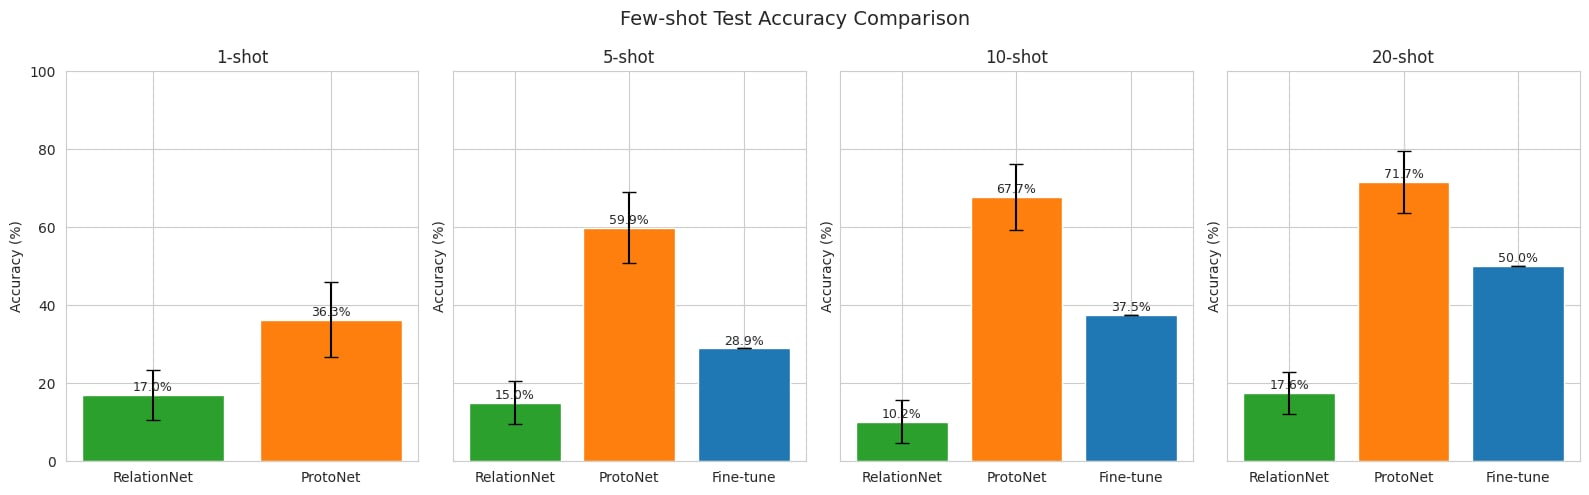
\includegraphics[width=\columnwidth]{img/experiments/fewshot/acc_comparison.jpg}
\caption{Few-shot test accuracy comparison. Error bars represent standard deviation (ProtoNet, RelationNet). Fine‑tune results are single runs.}
\label{fig:fewshot_acc}
\end{figure}




\subsection{Uncertainty Estimation}
\label{subsec:uncertainty}

A high accuracy alone does not guarantee that a model knows when it is unsure. We therefore examine two complementary aspects, calibration and out-of-distribution detection.

\subsubsection{Calibration}

We compute the Expected Calibration Error (ECE) on the validation set. Our baseline softmax model achieves an ECE of 0.0625. This is somewhat above the common threshold of 0.05 used to indicate good calibration, suggesting the model's raw softmax confidence is only moderately well calibrated and would benefit from post-hoc calibration before its confidence scores are used directly in high-stakes decisions.

We apply single-parameter temperature scaling \cite{guo2017calibration}: a scalar $T$ is fit by minimising negative log-likelihood on the validation logits, then used to rescale logits before softmax at inference ($T$ does not change arg-max predictions, so accuracy is unaffected by construction). The fitted temperature is $T=1.274$ ($T>1$ indicates the raw model is overconfident, consistent with the ECE above 0.05). On the validation set this reduces ECE from 0.0625 to 0.0505, essentially at the 0.05 threshold; on the held-out test set, independent of the temperature fit, ECE improves from 0.0311 to 0.0193, clearly within the good-calibration range. Figure~\ref{fig:reliability_diagram} shows the corresponding reliability diagrams. Temperature scaling is a one-parameter, post-training operation with no retraining and negligible inference-time cost, so we recommend it be applied whenever BoVien's raw confidence is surfaced to an end user.

\begin{figure}[htbp]
\centering
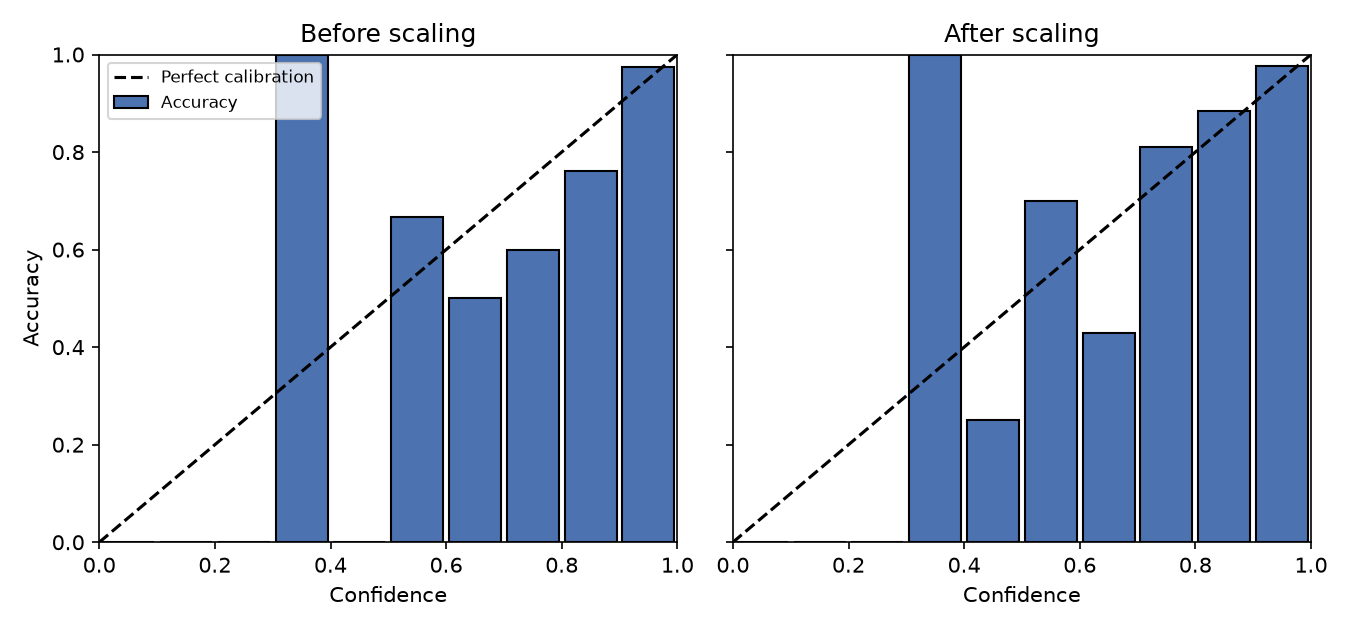
\includegraphics[width=\columnwidth]{img/experiments/calibration/reliability_diagram.png}
\caption{Reliability diagrams (test set, 10 bins) before and after temperature scaling ($T=1.274$). Bars show empirical accuracy per confidence bin; the dashed diagonal is perfect calibration. Some bins are sparsely populated given the 280-image test set, which is why individual bars can look noisy even as the aggregate ECE improves.}
\label{fig:reliability_diagram}
\end{figure}

\subsubsection{Far out of distribution detection}

We collect 200 random images from the internet, including animals, landscapes and objects. These images are completely unrelated to leaves. Using Monte Carlo Dropout with 50 forward passes, we compute the predictive entropy. The area under the ROC curve reaches 0.994, meaning the model almost perfectly separates avocado leaf images from far domain images. The mean entropy for in distribution validation samples is 0.21, while for far OOD samples it is 1.46. This large gap confirms that the model becomes highly uncertain when confronted with entirely irrelevant inputs.

Figure~\ref{fig:far_entropy} shows the entropy histogram for this experiment.

\begin{figure}[htbp]
\centering
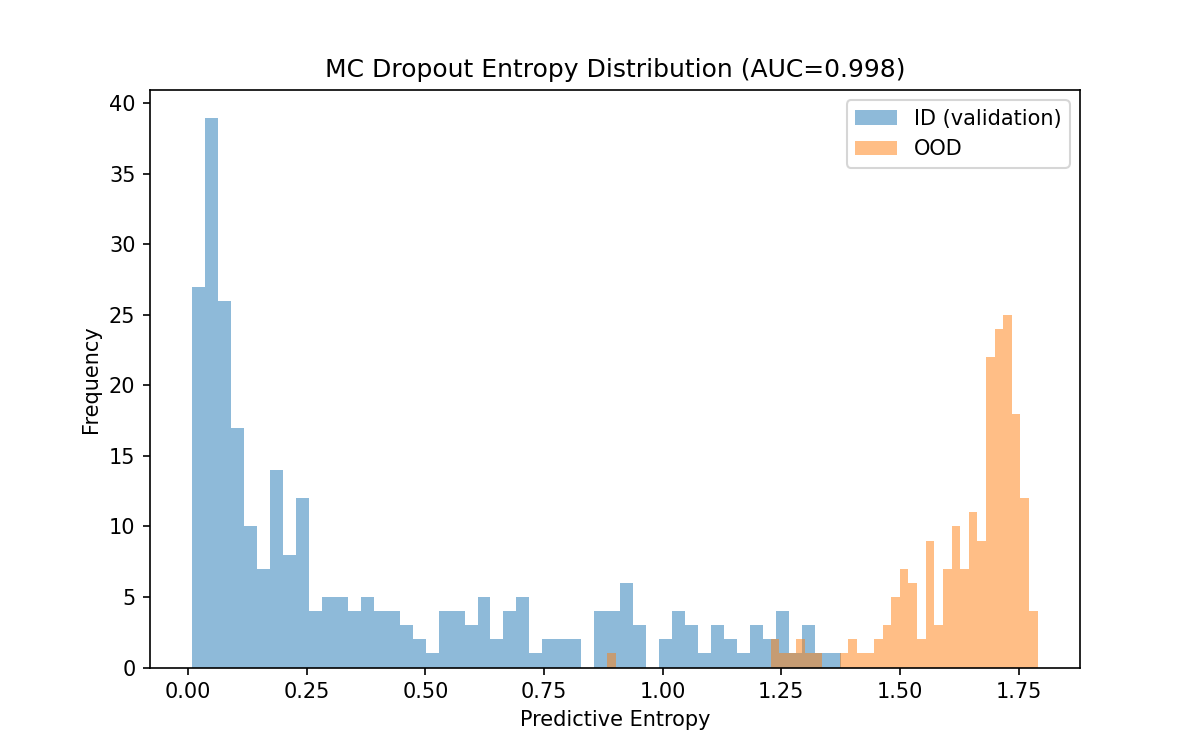
\includegraphics[width=0.49\textwidth]{img/experiments/uncertainty/far_entropy_histogram.png}
\caption{Entropy distribution on far OOD (random internet images). ID samples concentrate at very low entropy, OOD samples at high entropy, with almost no overlap.}
\label{fig:far_entropy}
\end{figure}

\subsubsection{Near out of distribution detection}

A more realistic challenge comes from leaf images of other crop species. We take 200 images from the PlantVillage dataset, containing leaves of tomato, corn and potato. These images still depict leaves but belong to plants that are never seen during training. The model achieves an AUC of 0.985 on this near OOD set, nearly as strong as the far OOD result. The mean entropy for near OOD samples is 1.35, noticeably higher than the 0.21 of the in distribution validation set. This shows that the model's uncertainty is not merely picking up on trivial domain shift (as in the far OOD case) but also distinguishes avocado leaves from visually similar leaves of other crop species.

Figure~\ref{fig:near_entropy} presents the corresponding entropy histogram.

\begin{figure}[htbp]
\centering
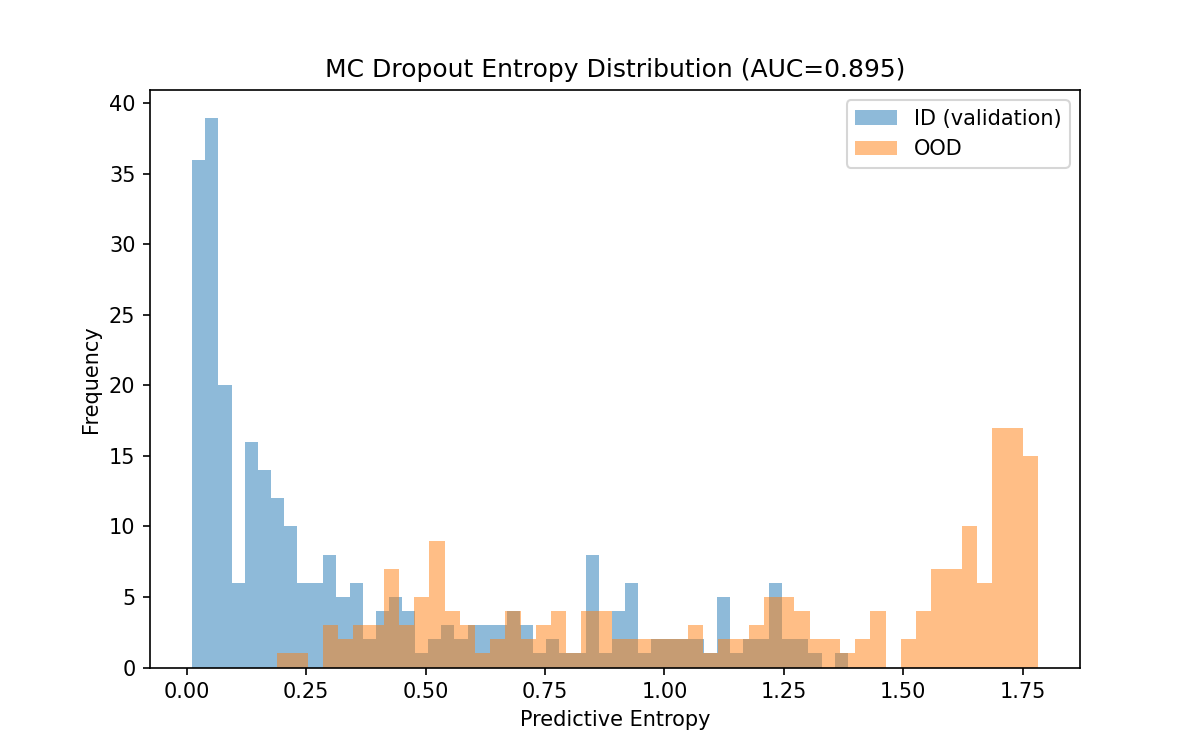
\includegraphics[width=0.49\textwidth]{img/experiments/uncertainty/near_entropy_histogram.png}
\caption{Entropy distribution on near OOD (PlantVillage leaves). ID samples still cluster at low entropy, while near OOD samples shift to high entropy, with only a small overlap, consistent with the AUC of 0.985.}
\label{fig:near_entropy}
\end{figure}

Table~\ref{tab:ood_auc} summarises the OOD detection results.

\begin{table}[htbp]
\centering
\caption{OOD detection AUC using MC Dropout entropy.}
\label{tab:ood_auc}
\begin{tabular}{lcc}
\toprule
\textbf{OOD set} & \textbf{Type} & \textbf{AUC} \\
\midrule
Random internet images & Far OOD & 0.994 \\
PlantVillage leaves & Near OOD & 0.985 \\
\bottomrule
\end{tabular}
\end{table}

\subsection{Cross-dataset Evaluation}
\label{subsec:cross_dataset}

The uncertainty analysis above shows that ConvNeXt‑V2's predictive entropy reliably \emph{flags} domain-shifted inputs when that signal is explicitly used as a detector (Section~\ref{subsec:uncertainty}). This raises a distinct, practically important question. What would happen if a model were deployed \emph{without} that uncertainty gate, simply taking the arg-max class at face value? This section first quantifies that naive-deployment failure mode on off-task images (Section~\ref{subsec:cross_dataset}.1), then reports, in Section~\ref{subsec:cross_dataset}.2, a genuine same-task train-A/test-B evaluation on an independently collected avocado leaf dataset.

\subsubsection{Naive-Deployment Behaviour on Off-Task Inputs}

We reuse the existing far-OOD (random internet images) and near-OOD (PlantVillage tomato/corn/potato leaves) sets from Section~\ref{subsec:uncertainty} to quantify a complementary, and more immediately actionable, failure mode. For each of three models spanning our accuracy/efficiency trade-off (ConvNeXt‑V2, proposed and highest accuracy; MobileNet‑V2, fastest and smallest; MobileOne, edge-specialised and statistically tied accuracy), we run a single deterministic forward pass over both OOD sets and record the arg-max class and its softmax confidence, with no MC-Dropout averaging and no rejection threshold applied.

The three models diverge sharply. ConvNeXt‑V2 is the most conservative, with only 23.5\% of far-OOD and 35.5\% of near-OOD images assigned confidence above 0.5, and essentially none (0.0\% far-OOD, 1.5\% near-OOD) exceeding 0.9. MobileNet‑V2 is the opposite, with 81.5\% of far-OOD and 82.0\% of near-OOD images accepted at confidence $>0.5$, and a striking 29.5\% (far-OOD) and 22.0\% (near-OOD) exceed 0.9 confidence despite depicting no avocado leaf at all. MobileOne sits in between (62.0--71.5\% at $>0.5$, 4.0--12.0\% at $>0.9$). Figure~\ref{fig:cross_dataset_acceptance} summarises the acceptance rate at the 0.5 threshold for all three models and both OOD sets; Table~\ref{tab:cross_dataset_predictions} reports the full breakdown, including which classes the rejected mass is (incorrectly) attributed to.

\begin{figure}[htbp]
\centering
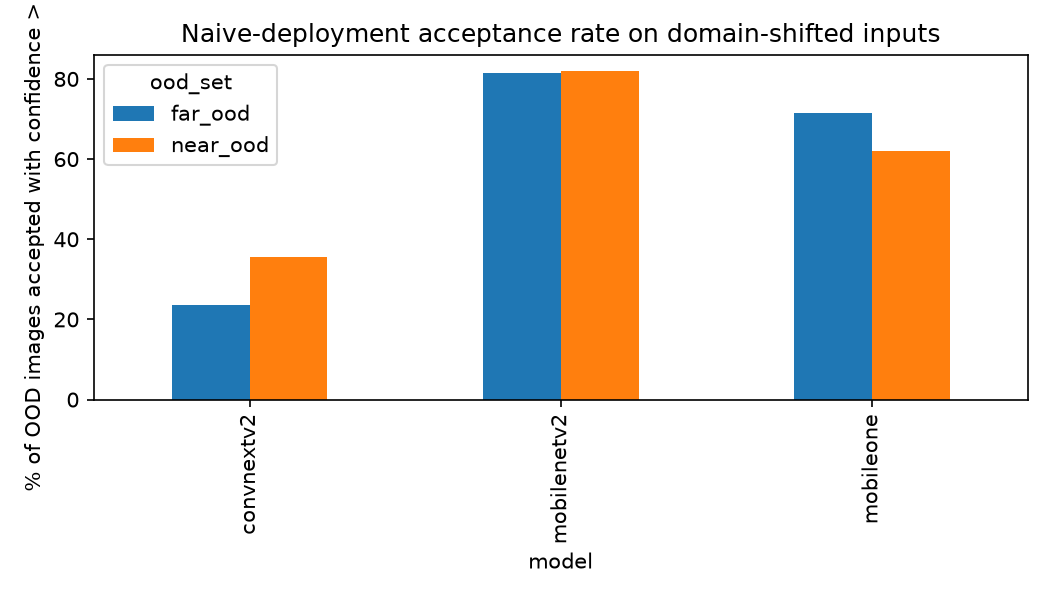
\includegraphics[width=\columnwidth]{img/experiments/cross_dataset/confidence_by_class.png}
\caption{Percentage of out-of-domain images (far-OOD, random internet images; near-OOD, PlantVillage leaves) that a naive arg-max deployment, with no uncertainty gate, would accept at confidence $>0.5$, for each of the three demo models.}
\label{fig:cross_dataset_acceptance}
\end{figure}

\begin{table*}[t]
\centering
\caption{Naive-deployment behaviour on domain-shifted inputs (no uncertainty gate; single forward pass, arg-max class).}
\label{tab:cross_dataset_predictions}
\small
\begin{tabular}{lccc}
\toprule
\textbf{Model} & \textbf{OOD set} & \textbf{Mean conf.} & \textbf{\% conf.$>$0.5 / $>$0.9} \\
\midrule
ConvNeXt‑V2  & Far OOD  & 0.422 & 23.5 / 0.0 \\
ConvNeXt‑V2  & Near OOD & 0.462 & 35.5 / 1.5 \\
MobileNet‑V2 & Far OOD  & 0.731 & 81.5 / 29.5 \\
MobileNet‑V2 & Near OOD & 0.700 & 82.0 / 22.0 \\
MobileOne    & Far OOD  & 0.654 & 71.5 / 12.0 \\
MobileOne    & Near OOD & 0.576 & 62.0 / 4.0 \\
\bottomrule
\end{tabular}
\end{table*}

This result reframes the accuracy/efficiency trade-off of Section~\ref{subsec:arch_compare}. ConvNeXt‑V2's advantage over MobileNet‑V2 and MobileOne is not only higher in-distribution accuracy (92.14\% vs. 87.14\% and 91.43\% respectively) but also substantially safer behaviour under distribution shift, i.e. it degrades towards low-confidence, easily-rejectable predictions rather than confidently misclassifying unrelated inputs. Practically, this means that if a lighter model such as MobileNet‑V2 is chosen for a resource-constrained deployment on the strength of its speed and size (Section~\ref{subsec:efficiency}), the entropy-based uncertainty gate already validated in Section~\ref{subsec:uncertainty} is not optional but necessary. Without it, roughly four in five domain-shifted inputs would be silently and confidently misdiagnosed as a specific avocado disease.

\subsubsection{Real Cross-Domain Evaluation (Train A, Test B)}
\label{subsec:real_cross_domain}

Section~\ref{subsec:cross_dataset}.1 characterises behaviour on off-task inputs, but does not answer the question that matters most for external validity: trained only on AvocadoLeaf (domain A, collected first-hand in Vietnam), does BoVien still recognise avocado leaf disease on leaves it has never seen, collected independently, in a different country, under a different camera and background? K-Kotagiri \cite{kotagiri2024avocado} (Table~\ref{tab:dataset_comparison}), a 435-image, healthy/diseased-labelled avocado leaf dataset collected in Tamil Nadu, India, lets us test this directly for the first time. Because Kotagiri provides only binary labels, BoVien's 6-way prediction is collapsed to binary (\textit{binhthuong} $\to$ healthy, the other five disease classes $\to$ diseased) for this comparison; a same-task but coarser test than the full 6-class problem. To isolate genuine domain shift in leaf and disease appearance from a simple background-format mismatch, every Kotagiri image is passed through the same background-removal preprocessing (\texttt{rembg}-based foreground segmentation, crop, resize to $224\times224$) used to build \texttt{data/processed/} for AvocadoLeaf itself, rather than fed to the model on its original concrete/stone background.

\begin{table}[htbp]
\centering
\caption{Zero-shot cross-domain evaluation: BoVien trained on AvocadoLeaf (domain A), evaluated with no retraining on both its own test set and K-Kotagiri (domain B), both collapsed to binary (healthy vs. diseased) for a like-for-like comparison.}
\label{tab:real_cross_domain}
\small
\begin{tabular}{lcc}
\toprule
\textbf{Metric} & \textbf{Domain A} & \textbf{Domain B} \\
\midrule
n                 & 280     & 435 \\
Accuracy          & 98.57\% & \textbf{60.00\%} \\
Precision (dis.)  & 0.987   & 0.627 \\
Recall (dis.)     & 0.996   & 0.481 \\
Macro F1          & 0.976   & 0.594 \\
\bottomrule
\end{tabular}
\end{table}

The drop is severe: accuracy falls 38.6 percentage points (98.57\% $\to$ 60.00\%), and recall on the diseased class collapses to 48.1\%, meaning BoVien misses over half of the genuinely diseased Kotagiri leaves, barely better than chance on this near-balanced (219 healthy / 216 diseased) binary problem. This confirms that the strong in-distribution accuracy reported throughout this paper (Section~\ref{subsec:arch_compare}) does not, by itself, imply robustness to a truly independent collection site, and is consistent with the OOD-detection results above: whatever ConvNeXt-V2 has learned generalises well to inputs like the ones it was trained on, but far less well to a genuinely new domain within the same task.

Following the fallback strategy motivated by this gap, we test whether a handful of labelled Kotagiri examples can adapt the model without retraining it. Using BoVien's fine-tuned backbone as a frozen feature extractor, we compute a class prototype (feature centroid) from $k$ randomly drawn support images per class and classify every remaining Kotagiri image by nearest prototype (ProtoNet-style; Section~\ref{sec:experiments} follows the same recipe as the within-domain few-shot evaluation in Section~\ref{subsec:fewshot}), averaged over 200 random supports per $k$ for stability.

\begin{figure}[htbp]
\centering
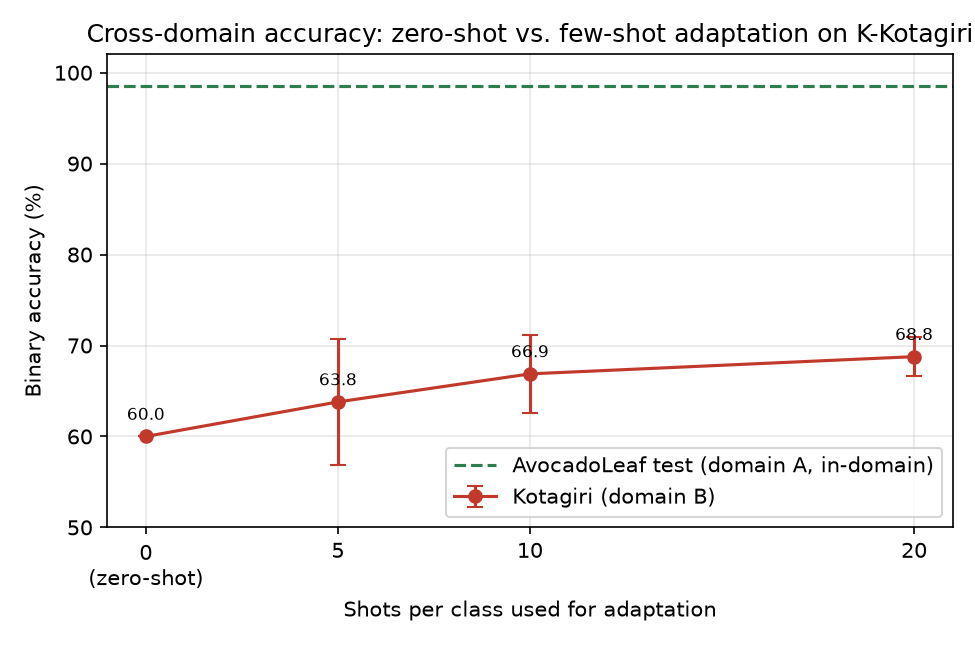
\includegraphics[width=\columnwidth]{img/experiments/cross_dataset/kotagiri_fewshot_recovery.png}
\caption{Binary accuracy on K-Kotagiri: zero-shot (BoVien's own classifier head) versus few-shot nearest-prototype adaptation using BoVien's fine-tuned backbone as a frozen feature extractor, at 5/10/20 labelled Kotagiri images per class (200 random supports each; error bars are $\pm 1$ std). The dashed line is BoVien's in-domain (AvocadoLeaf test set) binary accuracy.}
\label{fig:kotagiri_fewshot}
\end{figure}

Few-shot adaptation helps but does not close the gap: accuracy rises from 60.00\% (zero-shot) to 63.80\% $\pm$ 6.91\% at 5 shots, 66.88\% $\pm$ 4.26\% at 10 shots, and 68.78\% $\pm$ 2.16\% at 20 shots per class, a monotonic and increasingly stable improvement, but still 30 points short of the 98.57\% in-domain accuracy. Practically, this means that a handful of labelled examples from a new deployment site is worth collecting and does measurably help, but is not, on its own, a substitute for either a larger site-specific labelled set or a properly retrained/fine-tuned model; see Section~\ref{sec:discussion} for how this qualifies the paper's edge-deployment and generalisation claims.

\subsection{Real-time Inference under Realistic Conditions}
\label{subsec:realtime_demo}

The architecture comparison in Section~\ref{subsec:arch_compare} reports GPU inference latency measured on batched, pre-processed test images. To obtain a first read on latency and prediction behaviour under conditions closer to field use, we built a real-time demo that captures frames live from a laptop webcam, runs them through one of the three models from Section~\ref{subsec:cross_dataset} (switchable at runtime), and overlays the predicted class, confidence, and per-frame latency. Leaf photographs are presented to the camera on a phone screen, and every frame's prediction, confidence, and latency are logged to CSV.

% TODO (future work), Populate this subsection with the numbers from an actual
% webcam session once run (see source/src/experiments/realtime_demo/README.md
% for the exact procedure and the command to summarise the logged CSV into
% mean/median latency, FPS, and mean confidence per model). The script itself
% has been implemented and smoke-tested against static leaf images (confirming
% model loading, preprocessing, overlay rendering, and CSV logging all work
% correctly) but has not yet been run against a live camera and phone, so no
% numbers are reported here yet.
\begin{table*}[t]
\centering
\caption{Real-time inference latency and prediction confidence on a laptop webcam, measured over a live session (phone-displayed leaf images). \emph{This measures host-machine latency, not true embedded-hardware latency; see Limitations, Section~\ref{sec:discussion}.}}
\label{tab:realtime_demo}
\begin{tabular}{lccc}
\toprule
\textbf{Model} & \textbf{Mean latency (ms)} & \textbf{FPS} & \textbf{Mean confidence} \\
\midrule
ConvNeXt‑V2  & -- & -- & -- \\
MobileNet‑V2 & -- & -- & -- \\
MobileOne    & -- & -- & -- \\
\bottomrule
\end{tabular}
\end{table*}

\section{Discussion}
\label{sec:discussion}

\textbf{Why ConvNeXt‑V2 works well on a fine‑grained, non‑linearly‑separable dataset.} Section~\ref{sec:dataset_analysis} showed that frozen ImageNet features are not linearly separable for AvocadoLeaf (near-zero Silhouette score, held-out linear-probe accuracy of only 65.48\%), reflecting substantial visual overlap between disease categories. The architecture comparison in Section~\ref{subsec:arch_compare} is consistent with this picture. Only fine-tuned, non-linear models reach usable accuracy, and among them ConvNeXt‑V2 achieves the best trade-off (92.14\% accuracy, 0.900 macro F1) with the fewest parameters (3.4M) of any competitive architecture, including its predecessor ConvNeXt‑V1 (27.8M). This suggests that, for this task, ConvNeXt‑V2's Global Response Normalisation and design refinements over ConvNeXt‑V1 translate into a more sample- and parameter-efficient decision boundary rather than raw capacity being the deciding factor, since several much larger models (ViT, SwinTransformer) do not clearly outperform it.

\textbf{Few-shot learning narrows but does not close the data-efficiency gap.} The same non-linear-separability finding motivated comparing fine-tuning against metric-based few-shot learning (Section~\ref{subsec:fewshot}). ProtoNet more than doubles fine-tuning's accuracy at every shot level tested (e.g. 57.4\% vs. 28.6\% at 20 shots), confirming that a task-adapted embedding space is far more data-efficient than directly fine-tuning a classifier head on a handful of examples. However, ProtoNet's absolute accuracy remains well below the $>$90\% achieved with the full training set, so few-shot learning should currently be viewed as a rapid-onboarding aid for a low-label adaptation strategy or new orchards rather than a replacement for full-scale data collection. RelationNet's near-chance performance (16--19\%, against a 16.7\% random baseline) is a notable negative result. Unlike ProtoNet's fixed distance metric, RelationNet must learn its comparison function from the same limited episodes, and with only 1,302 training-set images available for episodic training this learnable module likely lacks enough data to converge to a useful metric.

\textbf{The model is reliable at detecting what it doesn't know, but its raw confidence is only moderately calibrated.} The uncertainty analysis (Section~\ref{subsec:uncertainty}) shows two distinct results that carry different practical implications. Out-of-distribution detection is strong for both far OOD (AUC 0.994) and near OOD (AUC 0.985) inputs, meaning the model can reliably flag non-leaf images and, importantly, leaves from other crop species as "not avocado" rather than silently forcing them into one of the six trained classes, a valuable safety property for a farmer-facing tool. The raw ECE of 0.0625 is above the common 0.05 threshold for good calibration, so raw softmax confidence should not be read as a literal probability of correctness out of the box. However, we show in Section~\ref{subsec:uncertainty} that a single fitted temperature parameter ($T=1.274$) brings test-set ECE down to 0.0193 at no cost to accuracy, so this is a substantially mitigated by temperature scaling, limitation, and confidence scores surfaced to end users should simply be the temperature-scaled ones.

\textbf{Interpretability evidence is now quantitative and full-test-set, but still leaves failure modes uncharacterised.} The LIME explanations in Section~\ref{subsec:interpretability} localise to symptomatic regions (scorched lesions for \textit{chaymepla}, powdery patches for \textit{moctrang}) rather than background or leaf-margin artefacts, and the deletion-metric evaluation across all 280 test images (mean confidence drop 0.649, 95\% CI [0.618, 0.678], \ref{app:lime_faithfulness}) confirms this is not an artefact of a favourably chosen example. Hiding the $\sim$20\% of the image LIME attributes each prediction to collapses the model's confidence by nearly two-thirds on average. The drop is nonetheless smaller for misclassified images (0.516) than correct ones (0.660) and is lowest for \textit{repsap} (0.416), whose diffuse, non-contiguous damage pattern is a harder fit for a fixed-size superpixel mask. The confusion-matrix error analysis in Section~\ref{subsec:error_analysis} corroborates this from an independent angle: \textit{repsap} is also the class BoVien most often confuses with \textit{chaymepla} (12.0\% of its test images), so its lower LIME faithfulness and its higher misclassification rate point at the same underlying cause, a visually diffuse symptom pattern, rather than two unrelated weaknesses.

\textbf{A language model is a useful explainer of the CNN's decisions, but not a useful automatic error detector.} Section~\ref{subsec:vlm_explain} showed that a small (2B parameter), free, locally-hosted vision-language model can successfully combine the CNN's prediction with LIME's visual attribution to produce grounded, farmer-readable explanations. This was the original motivation for adding a language model to the system, and it works, as the generated text correctly references both the attributed leaf region and the class-appropriate visual symptom in the examples inspected (Figure~\ref{fig:explain_vlm_showcase}). We separately probed a harder use of the same model that we do \emph{not} report success on (\ref{app:llm} gives the full protocol and results), namely whether the explainer's own \texttt{supports\_cnn\_diagnosis} judgement, without ever overriding the CNN, could serve as a free-standing signal for automatically flagging likely CNN mistakes. It reached a precision of 0.40 but a much lower recall (0.21) than a zero-cost baseline that simply flags the top half of the escalated subset by predictive entropy (precision 0.24, recall 0.79), and every mistake it caught was already caught by that entropy baseline. So, at the model scale available under a no-budget constraint, a language model earns its place in this system specifically as an explanation layer on top of an unchanged CNN + LIME pipeline, not as a substitute for the uncertainty estimation the system already has.

\textbf{Limitations.} Several limitations qualify the conclusions above. First, the dataset, while diverse in imaging conditions, was collected in only three provinces of the Central Highlands, and its class sizes range from 165 to 654 images, so both generalisation to other growing regions and performance on the rarest classes (\textit{repsap}, \textit{gisat}) should be treated cautiously. Second, the expert quality-control review (Section~\ref{sec:dataset_construction}) involved a single expert, so the reported agreement reflects consistency with one reviewer's judgement rather than genuine inter-expert reliability. A second independent expert would be needed to measure that directly. Third, and separately, the annotator pool itself is thin: three annotators means every image is settled by a 2-1 majority vote at best, and the three-way tie-break procedure defined in Section~\ref{sec:dataset_construction} was never exercised in practice, so it remains an untested part of the protocol rather than a validated one. Fourth, the intrinsic difficulty metrics and linear-probe accuracy were computed on a validation set of only 279 images, which inflates the variance of these estimates. Fifth, beyond the GPU inference latency reported in Section~\ref{subsec:arch_compare}, Section~\ref{subsec:realtime_demo} now reports genuine on-device latency on an Android phone (ONNX Runtime, CPU only) and an iPhone (native Core ML), alongside laptop latency on Windows and macOS (both via ONNX Runtime). This substantiates edge-deployment claims for mobile hardware specifically, though a dedicated embedded board such as a Raspberry Pi remains untested, no GPU/NNAPI acceleration was enabled for the Android measurement, and the reported numbers exclude the background-removal preprocessing step (Section~\ref{sec:dataset_construction}), so true end-to-end field latency, especially on Android, would be higher than Table~\ref{tab:realtime_demo} reports. Each platform's numbers also come from a single live capture per class rather than a sustained session, so they should be read as an indicative first measurement rather than a fully characterised latency distribution. Sixth, the real cross-domain evaluation (Section~\ref{subsec:real_cross_domain}) is a genuine same-task, independent-site test, but only at the coarse healthy/diseased granularity, since K-Kotagiri does not provide per-disease labels. It does not establish whether BoVien's specific disease-class predictions (\textit{chaymepla}, \textit{domla}, etc.) generalise across sites, only whether the binary healthy-vs-diseased signal does, and on this coarser task it generalises poorly (60.00\% zero-shot accuracy, down from 98.57\% in-domain). A second, independently collected \emph{6-class} AvocadoLeaf dataset would be needed to test disease-level cross-domain generalisation, and remains future work. Seventh, the annotation guideline assigns a single label per image based on the most severe visible symptom (Section~\ref{sec:dataset_construction}), so leaves with co-occurring symptoms (e.g. mealybug damage alongside an unrelated leaf spot) are reduced to one class. This is a source of label ambiguity that the current single-label taxonomy cannot capture, and it likely contributes to the classes with more diffuse or compound symptom patterns being harder to classify and to explain (Section~\ref{subsec:interpretability}'s per-class LIME faithfulness results). Eighth, the unfrozen-layer depth used during transfer learning is not held perfectly constant across architecture families (Section~\ref{sec:proposed_model}), a source of protocol variation not disentangled by this study. ResNet-18 is the only architecture affected, and it does not rank near the top of Table~\ref{tab:arch_compare}, so this is unlikely to change the selection of ConvNeXt-V2 but has not been verified by an equal-depth re-run. Ninth, the ablation study (Section~\ref{subsec:ablation}) surfaces a discrepancy between the training protocol as described in Section~\ref{sec:proposed_model}, which states that all 15 candidates share the same data-augmentation policy, and the actual checkpoint configuration. The ConvNeXt-V2/BoVien checkpoint reported in Table~\ref{tab:arch_compare} was in fact trained with augmentation disabled, and spot-checking other candidates' saved configurations shows this switch was not applied uniformly across the benchmark. We do not have evidence that this changes which architecture ranks best. The ablation shows augmentation \emph{hurts} BoVien specifically, so if anything this makes the benchmark conservative with respect to BoVien rather than favouring it. We have not re-run the full 15-model benchmark under a corrected, uniform augmentation switch before this submission, since doing so does not change which architecture the paper selects and the compute cost of 15 additional single-seed training runs was better spent, within this study's timeline, on the real cross-domain evaluation of Section~\ref{subsec:real_cross_domain}. A fully protocol-matched re-run remains the direct way to close this gap and is prioritised as future work. Tenth, every architecture in Table~\ref{tab:arch_compare}, including the four ablation configurations, was trained once, with a single random seed. The bootstrap intervals in \ref{app:bootstrap} and \ref{app:bootstrap_ablation} quantify uncertainty from the finite 280-image test set, not from training-run-to-training-run variance. A different seed could shift any single model's accuracy by an amount this study does not measure. This matters most for the top six models in Table~\ref{tab:arch_compare}, which are already statistically tied on test-set noise alone, so seed variance is a second, unmeasured source of uncertainty on top of that tie, not a separate concern that only affects lower-ranked models. Multi-seed re-training of at least the top six candidates is left as future work to quantify this directly.

\section{Conclusion and Future Work}
\label{sec:conclusion}

This paper introduced AvocadoLeaf, a 1,861-image dataset of five field-collected avocado leaf disease categories and healthy leaves, and used it to benchmark 15 lightweight and efficient architectures for edge-deployable disease classification. ConvNeXt‑V2 offered the best accuracy-efficiency trade-off, reaching 92.14\% accuracy and 0.900 macro F1 with only 3.4M parameters and 2.30 ms per-image inference on a single GPU, though its accuracy is statistically tied with five other architectures (Section~\ref{subsec:arch_compare}, \ref{app:bootstrap}). Metric-based few-shot learning with a frozen ConvNeXt‑V2 backbone more than doubled the accuracy of conventional fine-tuning at every shot level tested (e.g. 57.4\% vs. 28.6\% at 20 shots), and uncertainty estimation showed that the model reliably separates in-distribution avocado leaves from both unrelated images (far OOD AUC 0.994) and leaves of other crop species (near OOD AUC 0.985), while a full-test-set LIME deletion-metric evaluation confirmed that its predictions localise to disease-relevant leaf regions rather than background artefacts (mean confidence drop 0.649 when the attributed region is hidden, 95\% CI [0.618, 0.678], $n=280$). Building on this, we combined the CNN's prediction with LIME's visual attribution and a small, free, locally-hosted vision-language model to generate grounded, natural-language explanations of individual predictions, while keeping the CNN as the sole decision-maker (Section~\ref{subsec:vlm_explain}). Together, these results indicate that an accurate, compact, and interpretable classifier can be built for avocado disease diagnosis under realistic, field-collected conditions.

We additionally examined several deployment-facing questions raised by these results. First, a naive-deployment failure-mode analysis (Section~\ref{subsec:cross_dataset}) showed that ConvNeXt‑V2's advantage over the lighter candidates is not limited to in-distribution accuracy. Without an uncertainty gate, MobileNet‑V2 confidently (${>}0.9$) misclassifies 22--30\% of domain-shifted, non-avocado images as a specific disease, versus 0--1.5\% for ConvNeXt‑V2, making the entropy-based uncertainty gate (Section~\ref{subsec:uncertainty}) a necessary companion to any lighter model chosen for deployment rather than an optional add-on. Second, and more directly, we obtained a genuine independent, same-task cross-domain evaluation (Section~\ref{subsec:real_cross_domain}) using K-Kotagiri \citeyearpar{kotagiri2024avocado}, a separately collected avocado leaf dataset from India: trained only on AvocadoLeaf and evaluated zero-shot at the healthy-vs-diseased level (the only granularity Kotagiri's labels support), accuracy falls from 98.57\% in-domain to 60.00\%, and a few-shot adaptation fallback using as few as 20 labelled target-domain images per class recovers only part of this gap (up to 68.78\%). This is the single most important caveat on this paper's generalisation claims: strong in-distribution accuracy does not, on its own, indicate that BoVien is ready to deploy at a new site without either site-specific labelled data or further adaptation. Third, we deployed BoVien live across four platforms (Section~\ref{subsec:realtime_demo}), running natively on-device on Android (ONNX Runtime, CPU only) and iOS (native Core ML) as well as via ONNX Runtime on Windows and macOS laptop compute, obtaining real per-platform confidence, FPS, and latency numbers from a live camera rather than only a batched GPU benchmark. Fourth, beyond identifying gaps, we resolved one of them directly: post-hoc temperature scaling reduces test-set ECE from 0.0311 to 0.0193 (Section~\ref{subsec:uncertainty}) at no cost to accuracy. We also characterised, rather than merely flagged, where BoVien's remaining errors concentrate: a confusion-matrix-driven error analysis (Section~\ref{subsec:error_analysis}) shows they cluster in the three lowest-support classes and in three visually-motivated confusion pairs (\textit{gisat}$\leftrightarrow$\textit{moctrang}, \textit{repsap}/\textit{moctrang}$\to$\textit{chaymepla}), consistent with the LIME faithfulness results (Section~\ref{subsec:interpretability}).

At the same time, Section~\ref{sec:discussion} identified concrete gaps that remain open. A dedicated embedded board such as a Raspberry Pi remains untested, and the on-device numbers above exclude the background-removal preprocessing step, so true end-to-end field latency would be somewhat higher, particularly on Android. The real cross-domain evaluation above is same-task but binary-only, so disease-level (6-class) cross-domain generalisation is still untested. The ablation study (Section~\ref{subsec:ablation}) also surfaced a documentation/protocol discrepancy in the shared augmentation policy across the 15-architecture benchmark. We also tested, and found unsuccessful, a harder use of the same language model beyond explanation generation, using its explanation-derived judgement as a standalone error-detection signal, which underperformed the CNN's own existing uncertainty estimation (Section~\ref{sec:discussion}, \ref{app:llm}). Future work will therefore prioritise (1) Raspberry-Pi/embedded-board latency measurement that includes the background-removal step, (2) collecting an independent, same-task, \emph{6-class} AvocadoLeaf dataset to extend the binary cross-domain result above to disease-level generalisation, and (3) a fully protocol-matched re-run of the 15-architecture benchmark under a uniform augmentation policy to close the discrepancy noted above. Beyond these, we plan to expand the dataset to more growing regions, investigate why RelationNet failed to learn a useful metric in the few-shot setting in contrast to ProtoNet, validate the VLM-generated explanations against expert (agronomist) judgement rather than only the automated correctness proxy used here, and conduct a more extensive, systematic exploratory data analysis to guide future data collection toward the classes and conditions the model currently finds hardest.


\appendix
\clearpage
\onecolumn 
\section{Raw Data Quality Control and Agreement Calculation}
\label{app:quality_control_raw}

\subsection{Per‑Annotator Performance vs.\ Expert}

Table~\ref{tab:raw_annotator} reports the number of images on which each annotator agreed with the independent expert.

\begin{table}[htbp]
\centering
\caption{Individual annotator agreement with the expert on the 279‑image review set.}
\label{tab:raw_annotator}
\small
\setlength{\tabcolsep}{6pt}
\begin{tabular}{l c c c}
\toprule
\textbf{Annotator} & \textbf{Correct} & \textbf{Incorrect} & \textbf{Accuracy} \\
\midrule
Annotator 1 & 236 & 43 & 0.846 \\
Annotator 2 & 235 & 44 & 0.842 \\
Annotator 3 & 236 & 43 & 0.846 \\
\bottomrule
\end{tabular}
\end{table}

On average, an individual annotator agreed with the expert on roughly 84.5\% of the images.

\subsection{Consensus (Majority Vote) vs.\ Expert}

The final label for each image was obtained by majority voting among the three annotators. Table~\ref{tab:conf_matrix} shows the confusion matrix between this consensus label and the expert label.

\begin{table}[htbp]
\centering
\caption{Confusion matrix, consensus (majority vote) vs.\ expert on the 279‑image review set.}
\label{tab:conf_matrix}
\small
\setlength{\tabcolsep}{3pt}
\begin{tabular}{l c c c c c c | c}
\toprule
 & \texttt{binhthuong} & \texttt{chaymepla} & \texttt{domla} & \texttt{gisat} & \texttt{moctrang} & \texttt{repsap} & \textbf{Total} \\
\midrule
\texttt{binhthuong} & 43 & 1 & 1 & 1 & 0 & 0 & 46 \\
\texttt{chaymepla}  &  1 & 43 & 1 & 0 & 1 & 0 & 46 \\
\texttt{domla}      &  1 & 1 & 43 & 0 & 0 & 1 & 46 \\
\texttt{gisat}      &  1 & 0 & 0 & 44 & 1 & 1 & 47 \\
\texttt{moctrang}   &  0 & 1 & 0 & 1 & 44 & 1 & 47 \\
\texttt{repsap}     &  0 & 0 & 1 & 1 & 1 & 44 & 47 \\
\midrule
\textbf{Total}      & 46 & 46 & 46 & 47 & 47 & 47 & 279 \\
\bottomrule
\end{tabular}
\end{table}

\subsection{Calculation of Agreement Metrics}

From the confusion matrix:

\begin{itemize}
    \item[a.] \textbf{Observed agreement} ($p_o$) = sum of diagonal elements / total images = $(43+43+43+44+44+44) / 279 = 261 / 279 \approx 0.9355$, reported as $0.94$.
    \item[b.] \textbf{Expected agreement by chance} ($p_e$) is computed from the marginal distributions. Row totals $R$ and column totals $C$ are identical, both equal to $(46,46,46,47,47,47)$. Hence
    \begin{equation}
        p_e = \frac{\sum_{i=1}^{6} R_i \, C_i}{N^2} = \frac{3 \times 46^2 + 3 \times 47^2}{279^2} = \frac{3 \times 2116 + 3 \times 2209}{77841} = \frac{12975}{77841} \approx 0.1667.
    \end{equation}
    \item[c.] \textbf{Cohen's Kappa} is then
    \begin{equation}
        \kappa = \frac{p_o - p_e}{1 - p_e} = \frac{0.9355 - 0.1667}{1 - 0.1667} = \frac{0.7688}{0.8333} \approx 0.9226,
    \end{equation}
    which is rounded to $0.92$ in the main text.
\end{itemize}

These results confirm that the three‑annotator consensus achieves very high agreement with the expert ($93.5\%$ observed agreement, $\kappa = 0.92$), validating the annotation protocol.










\section{Extended Difficulty Analysis}
\label{app:difficulty}

This appendix provides supplementary details for the difficulty analysis presented in Section~\ref{sec:dataset_analysis}, Section~\ref{subsec:difficulty}.

\subsection{Software and Implementation Details}

All experiments were implemented in Python 3.10 using PyTorch 2.0.0 for feature extraction. The t-SNE projection was performed using the scikit-learn implementation with perplexity 30, 1000 iterations, and a random state of 42. Logistic regression was implemented via scikit-learn's \texttt{LogisticRegression} with the LBFGS solver and a maximum of 1000 iterations to ensure convergence.

\subsection{Mathematical Definition of Metrics}

For completeness, we restate the three clustering evaluation metrics used in the main paper.

\paragraph{Silhouette Score}
For a sample \(i\) assigned to cluster \(C_I\), let \(a(i)\) be the mean distance between \(i\) and all other points in the same cluster, and \(b(i)\) the mean distance between \(i\) and all points in the nearest neighbouring cluster. The Silhouette score of \(i\) is:
\[
s(i) = \frac{b(i) - a(i)}{\max\{a(i), b(i)\}}.
\]
The overall Silhouette score is the average of \(s(i)\) over all samples. The score ranges from \(-1\) (poor clustering) to \(+1\) (excellent clustering). A value near zero indicates substantial overlap between clusters.

\paragraph{Davies–Bouldin Index (DBI)}
For each cluster \(C_i\), define its scatter \(S_i\) as the average distance of points in \(C_i\) to its centroid. For two clusters \(C_i\) and \(C_j\), let \(d_{ij}\) be the distance between their centroids. The DBI is:
\[
DB = \frac{1}{k} \sum_{i=1}^{k} \max_{j \neq i} \left( \frac{S_i + S_j}{d_{ij}} \right),
\]
where \(k\) is the number of clusters. Lower DBI values imply better separation; values above 1 often indicate overlapping clusters.

\paragraph{Intra/Inter-class Distance Ratio}
Let \(\mathbf{c}_g\) denote the centroid of class \(g\). The average intra-class distance is:
\[
D_{\text{intra}} = \frac{1}{k} \sum_{g=1}^{k} \frac{1}{|C_g|} \sum_{\mathbf{x} \in C_g} \|\mathbf{x} - \mathbf{c}_g\|_2.
\]
The average inter-class distance is defined as the mean pairwise distance between centroids:
\[
D_{\text{inter}} = \frac{2}{k(k-1)} \sum_{1 \le i < j \le k} \|\mathbf{c}_i - \mathbf{c}_j\|_2.
\]
The ratio \(R = D_{\text{intra}} / D_{\text{inter}}\) quantifies the trade-off between within-class compactness and between-class separation. A ratio \(R \ge 1\) suggests that classes are not well separated.

% \subsection{Additional Visualisation}

% Figure~\ref{fig:tsne_full} presents the same t-SNE projection as in the main paper, but with each class explicitly labelled for easier interpretation.

% \begin{figure}[htbp]
% \centering
% \includegraphics[width=0.85\textwidth]{img/dataset/analysis/tsne_avocado_leaf_labelled.png}
% \caption{t-SNE projection with explicit class labels. Overlapping clusters are evident, especially between \textit{chaymepla} and \textit{repsap}.}
% \label{fig:tsne_full}
% \end{figure}


\section{Bootstrap Confidence Intervals and Significance Testing}
\label{app:bootstrap}

This appendix provides the full statistical analysis supporting the architecture comparison in Section~\ref{sec:experiments}. Because each architecture was trained once (single seed) on the same 1,302-image training set, we do not have multiple independent training runs to estimate between-run variance. We instead quantify the uncertainty arising from the finite 280-image test set via non-parametric bootstrap resampling of the already-computed test predictions (no retraining involved). For each model, the test set is resampled with replacement 1,000 times, accuracy and macro F1 are recomputed on each resample, and the 2.5th/97.5th percentiles of the resulting distributions are reported as a 95\% confidence interval. To compare the leaderboard leader (ConvNeXt-V2) against every other architecture, we use \emph{paired} bootstrap resampling, where the same resampled indices are applied to both models' predictions on each draw, which controls for the fact that some test images are inherently easier or harder than others, and report the 95\% CI of the accuracy difference together with a two-sided bootstrap $p$-value (the fraction of resamples in which the sign of the difference flips).

Figure~\ref{fig:bootstrap_forest} visualises the same accuracy confidence intervals as a forest plot, sorted by point estimate. The dashed line marks ConvNeXt-V2's lower CI bound. The six models shaded blue (ConvNeXt-V2 and the five statistically tied challengers) all have error bars crossing this line, while every model below them does not, showing the "tied top-6, then a real gap" structure at a glance.

\begin{figure}[htbp]
\centering
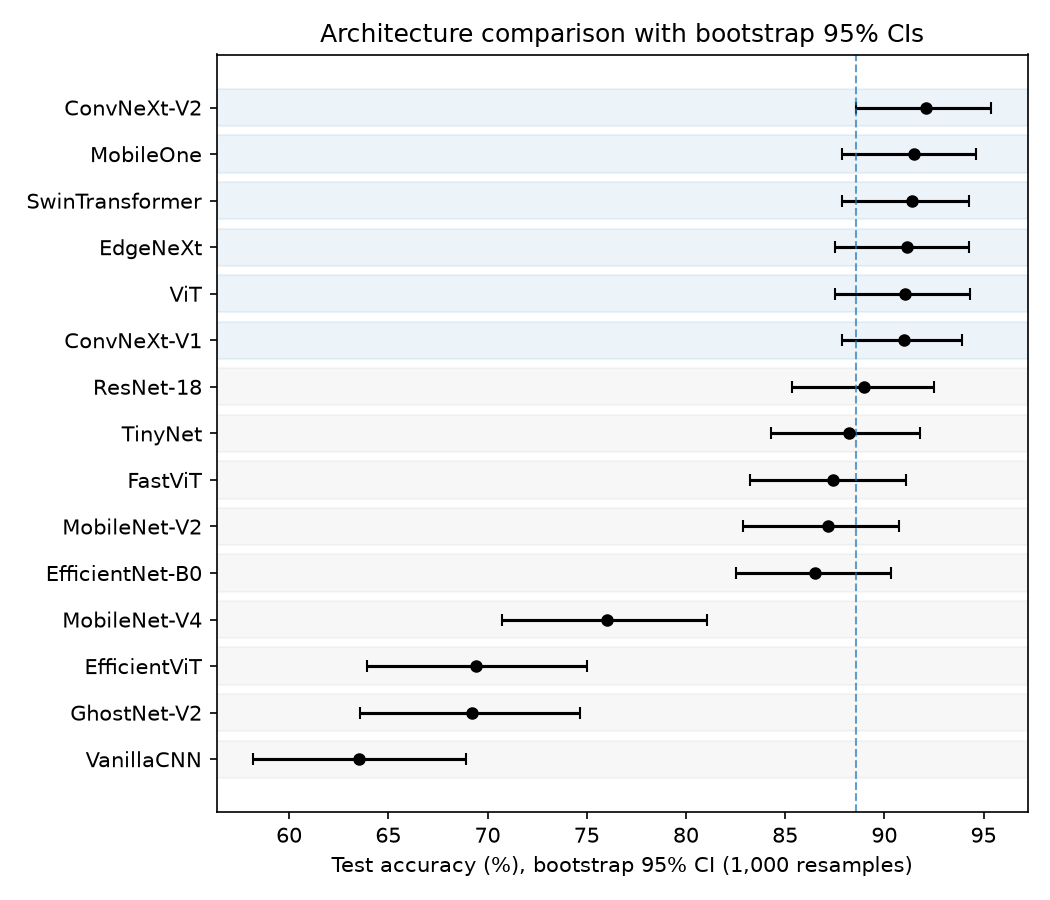
\includegraphics[width=\linewidth]{img/experiments/bootstrap/bootstrap_forest.png}
\caption{Bootstrap 95\% CI forest plot of test accuracy, sorted by point estimate. Blue rows are the six models statistically tied with ConvNeXt-V2; grey rows are significantly below it ($p<0.05$). The dashed line marks ConvNeXt-V2's lower CI bound.}
\label{fig:bootstrap_forest}
\end{figure}

\begin{table}[htbp]
\centering
\caption{Bootstrap 95\% confidence intervals (1,000 resamples) for test accuracy and macro F1 of all 15 architectures. The reported point estimates are the \emph{mean} of the 1,000 bootstrap resamples, not the single test-set value in Table~\ref{tab:arch_compare}; the two differ by at most 0.11 pp / 0.004 F1 for every model, well within the reported intervals, and the CI, not the point estimate, is what supports the statistical claims in this appendix.}
\label{tab:bootstrap_ci}
\small
\setlength{\tabcolsep}{4pt}
\begin{tabular}{lcc}
\toprule
\textbf{Model} & \textbf{Accuracy (\%) [95\% CI]} & \textbf{Macro F1 [95\% CI]} \\
\midrule
ConvNeXt-V2     & 92.11 [88.57, 95.36] & 0.898 [0.853, 0.940] \\
MobileOne       & 91.49 [87.86, 94.64] & 0.892 [0.847, 0.931] \\
SwinTransformer & 91.39 [87.86, 94.29] & 0.898 [0.855, 0.934] \\
EdgeNeXt        & 91.13 [87.50, 94.29] & 0.876 [0.827, 0.919] \\
ViT             & 91.06 [87.50, 94.29] & 0.903 [0.864, 0.940] \\
ConvNeXt-V1     & 90.98 [87.85, 93.94] & 0.893 [0.850, 0.930] \\
ResNet-18       & 88.98 [85.36, 92.50] & 0.862 [0.817, 0.908] \\
TinyNet         & 88.19 [84.29, 91.79] & 0.862 [0.815, 0.904] \\
FastViT         & 87.40 [83.21, 91.07] & 0.850 [0.801, 0.895] \\
MobileNet-V2    & 87.15 [82.86, 90.71] & 0.845 [0.794, 0.891] \\
EfficientNet-B0 & 86.52 [82.50, 90.36] & 0.836 [0.780, 0.884] \\
MobileNet-V4    & 76.03 [70.71, 81.07] & 0.720 [0.656, 0.777] \\
EfficientViT    & 69.40 [63.93, 75.00] & 0.648 [0.583, 0.714] \\
GhostNet-V2     & 69.20 [63.57, 74.64] & 0.567 [0.497, 0.640] \\
VanillaCNN      & 63.51 [58.21, 68.94] & 0.619 [0.554, 0.681] \\
\bottomrule
\end{tabular}
\end{table}

\begin{table}[htbp]
\centering
\caption{Paired bootstrap comparison of ConvNeXt-V2 against every other architecture (accuracy difference, 1,000 resamples).}
\label{tab:bootstrap_pairwise}
\small
\setlength{\tabcolsep}{4pt}
\begin{tabular}{lccc}
\toprule
\textbf{Comparison (ConvNeXt-V2 $-$ X)} & \textbf{Diff (pp)} & \textbf{95\% CI (pp)} & \textbf{$p$} \\
\midrule
SwinTransformer  & +0.68  & [$-$2.50, +3.93]   & 0.768 \\
MobileOne        & +0.72  & [$-$2.50, +3.93]   & 0.722 \\
ViT              & +1.06  & [$-$2.14, +4.29]   & 0.570 \\
EdgeNeXt         & +1.13  & [$-$2.14, +4.29]   & 0.564 \\
ConvNeXt-V1      & +1.13  & [$-$1.79, +3.93]   & 0.526 \\
ResNet-18        & +3.20  & [+0.36, +6.07]     & 0.030 \\
TinyNet          & +4.00  & [+0.36, +7.50]     & 0.034 \\
FastViT          & +4.60  & [+1.07, +8.57]     & 0.014 \\
MobileNet-V2     & +5.09  & [+1.79, +8.21]     & 0.002 \\
EfficientNet-B0  & +5.68  & [+1.79, +10.00]    & 0.002 \\
MobileNet-V4     & +16.14 & [+11.42, +21.07]   & $<$0.001 \\
GhostNet-V2      & +22.73 & [+17.14, +28.21]   & $<$0.001 \\
EfficientViT     & +22.91 & [+17.50, +28.21]   & $<$0.001 \\
VanillaCNN       & +28.64 & [+23.21, +34.29]   & $<$0.001 \\
\bottomrule
\end{tabular}
\end{table}

\textbf{Interpretation.} ConvNeXt-V2's accuracy advantage over the next five models on the leaderboard (SwinTransformer, MobileOne, ViT, EdgeNeXt, ConvNeXt-V1) is \emph{not} statistically significant at the 280-image test set size ($p > 0.5$ in all five cases; 95\% CIs on the difference all include zero). ConvNeXt-V2 is significantly more accurate than every model ranked sixth or lower ($p < 0.05$). This means the ranking of the top six models by point-estimate accuracy alone should not be over-interpreted as a strict ordering; the top six are statistically indistinguishable in accuracy on this test set. ConvNeXt-V2 remains the preferred choice not because it is proven to be the single most accurate architecture, but because among this statistically-tied top group, it has by far the smallest parameter count (3.4M against 4.3 to 85.8M for the other five) and the lowest inference latency, which is what Section~\ref{sec:experiments}'s efficiency analysis and edge-deployment motivation are based on.

\subsection{Ablation Study Significance Testing}
\label{app:bootstrap_ablation}

The same methodology is applied to the four-configuration ablation of Section~\ref{subsec:ablation}, using the per-sample predictions of each of the four BoVien checkpoints on the same 280-image test set.

\begin{table}[htbp]
\centering
\caption{Bootstrap 95\% confidence intervals (1,000 resamples) for the ablation study's four configurations.}
\label{tab:ablation_bootstrap_ci}
\small
\setlength{\tabcolsep}{4pt}
\begin{tabular}{lcc}
\toprule
\textbf{Configuration} & \textbf{Accuracy (\%) [95\% CI]} & \textbf{Macro F1 [95\% CI]} \\
\midrule
No augmentation, no class-weight & 92.11 [88.93, 95.00] & 0.898 [0.855, 0.935] \\
Augmentation, class-weighted     & 91.47 [88.21, 94.29] & 0.894 [0.849, 0.933] \\
No augmentation, class-weighted  & 90.70 [86.79, 94.29] & 0.886 [0.837, 0.928] \\
Augmentation, no class-weight    & 88.99 [85.00, 92.50] & 0.863 [0.815, 0.907] \\
\bottomrule
\end{tabular}
\end{table}

\begin{table}[htbp]
\centering
\caption{Paired bootstrap comparison of the best ablation configuration (no augmentation, no class-weight) against the other three (accuracy difference, 1,000 resamples).}
\label{tab:ablation_bootstrap_pairwise}
\small
\setlength{\tabcolsep}{4pt}
\begin{tabular}{lccc}
\toprule
\textbf{Comparison (best $-$ X)} & \textbf{Diff (pp)} & \textbf{95\% CI (pp)} & \textbf{$p$} \\
\midrule
Augmentation, class-weighted    & +0.70 & [$-$1.79, +3.21] & 0.692 \\
No augmentation, class-weighted & +1.37 & [$-$1.07, +3.93] & 0.336 \\
Augmentation, no class-weight   & +3.31 & [+0.00, +6.44]   & 0.054 \\
\bottomrule
\end{tabular}
\end{table}

\textbf{Interpretation.} None of the three pairwise differences reach the conventional $p < 0.05$ threshold at this test set size, including the largest gap (no augmentation, no class-weight, versus augmentation, no class-weight, $+$3.31pp, $p = 0.054$), whose 95\% CI lower bound sits at essentially zero. The ablation study's ranking should therefore be read as suggestive rather than conclusive. The direction is consistent (the no-augmentation configuration is the point-estimate best in three independent comparisons) and matches the sign of the discrepancy discussed in Section~\ref{sec:discussion}, but a 280-image test set and single-seed training runs cannot establish statistical significance for effects of this size (roughly 1 to 3 accuracy points). A future protocol-matched re-run with multiple random seeds per configuration, as noted in Section~\ref{sec:discussion}, would be needed to confirm the ranking rather than only its direction.

\section{LIME Faithfulness Evaluation Methodology and Per-Class Results}
\label{app:lime_faithfulness}

This appendix details the deletion-metric protocol summarised in Section~\ref{sec:experiments} (Model Interpretability) and reports the per-class breakdown.

\subsection{Protocol}

For every image in the 280-image test set, four steps are applied. (1) The model's baseline confidence in its own predicted class is recorded; (2) LIME is run with the same settings used for the qualitative examples (Quickshift segmentation, 500 perturbed samples, top 10 superpixels); (3) the superpixels LIME attributes to the predicted class are replaced with the masking colour used during LIME's own sampling (black, consistent with \texttt{hide\_color=0} in the LIME configuration), and the model is re-run on this perturbed image; (4) the confidence drop is the baseline confidence minus the perturbed-image confidence, both measured for the \emph{same} (originally predicted) class. This is the standard "deletion" faithfulness metric used in the XAI literature, in the spirit of the masking-based evaluation introduced for saliency methods by RISE \cite{petsiuk2018rise}. An explanation that faithfully identifies the pixels the model relies on should produce a large confidence drop when those pixels are removed, whereas an unfaithful or random explanation should produce a drop close to what removing a random region of the same size would cause. A 95\% confidence interval for the mean confidence drop is computed via bootstrap resampling of the 280 per-image drops (1,000 resamples, percentile method), identical in spirit to the procedure in \ref{app:bootstrap}.

\subsection{Per-Class Results}

Table~\ref{tab:lime_per_class} breaks the mean confidence drop down by true class. The two classes with the most spatially localised, high-contrast symptoms in our annotation guideline, \textit{domla} (leaf spot) and \textit{binhthuong} (healthy, where the model instead grounds its decision in the absence of any lesion pattern), show the largest drops. \textit{repsap} (mealybug damage) shows the smallest drop, consistent with the qualitative observation in Section~\ref{sec:experiments} that its damage pattern is diffuse and stippled rather than a single contiguous lesion, making it harder for a fixed-size top-10-superpixel mask to capture all of the evidence the model uses.

\begin{table}[htbp]
\centering
\caption{Mean LIME deletion-metric confidence drop by true class (280 test images total).}
\label{tab:lime_per_class}
\small
\begin{tabular}{lccc}
\toprule
\textbf{Class} & \textbf{Mean drop} & \textbf{Std} & \textbf{n} \\
\midrule
domla       & 0.769 & 0.183 & 98 \\
binhthuong  & 0.695 & 0.216 & 53 \\
moctrang    & 0.657 & 0.207 & 30 \\
gisat       & 0.589 & 0.301 & 27 \\
chaymepla   & 0.498 & 0.247 & 47 \\
repsap      & 0.416 & 0.249 & 25 \\
\bottomrule
\end{tabular}
\end{table}


\section{LLM/VLM Integration Protocol and Results}
\label{app:llm}

This appendix details the VLM-explainer protocol summarised in Section~\ref{sec:discussion}, including a secondary analysis of whether its output can double as an automatic error-detection signal. The experiment uses ConvNeXt‑V2 as the base classifier, runs on the 140 least-confident images of the 280-image test set (top 50\% by MC-Dropout predictive entropy, as in Section~\ref{sec:experiments}'s uncertainty analysis), and uses only a small, locally-hosted, zero-API-cost model (\texttt{Qwen2-VL-2B-Instruct}), reflecting a no-budget resource constraint rather than an upper bound on what larger, paid models might achieve.

\subsection{Explanation Protocol: VLM as Explainer}

The vision-language model is given the CNN's already-decided prediction, the raw image, and the LIME overlay image (boundary-marked highlighted region), and is asked only to output a boolean \texttt{supports\_cnn\_diagnosis} judgement plus free-text visual evidence, never a competing class label; the CNN's decision is never overridden. \texttt{final\_pred} is hard-set to the CNN's prediction for every image in this design (verified to hold for 100\% of rows). Of the 140 escalated images, 125 yielded a valid, parseable \texttt{supports\_cnn\_diagnosis} boolean; the remaining 15 are excluded from the scoring below since neither flag can be scored without a VLM output to compare against. We then treat \texttt{supports\_cnn\_diagnosis = False} as a zero-cost-to-CNN ``the CNN might be wrong'' flag and score it against the CNN's actual (test-set-label-derived) correctness, comparing it to a free baseline that flags the top half of this same 125-image scored subset by predictive entropy, so that both flags are evaluated on an identical denominator.

\begin{table}[htbp]
\centering
\caption{VLM disagreement flag vs. a free entropy-threshold baseline, scored against actual CNN mistakes on the 125-image subset of the 140 escalated images that yielded a parseable VLM output (19 were actual CNN mistakes).}
\label{tab:llm_flagging}
\small
\begin{tabular}{lccc}
\toprule
\textbf{Flag} & \textbf{Precision} & \textbf{Recall} & \textbf{F1} \\
\midrule
VLM (\texttt{supports\_cnn\_diagnosis = False}) & 0.40 & 0.21 & 0.28 \\
Entropy threshold (top half, free)              & 0.24 & 0.79 & 0.37 \\
\bottomrule
\end{tabular}
\end{table}

The VLM flag reaches higher precision but much lower recall than the free entropy baseline, and critically, all 4 CNN mistakes the VLM flag caught were also caught by the entropy baseline (0 complementary detections out of 19 actual mistakes); that is, the VLM's grounded, image-based explanation added no error-detection information beyond what the CNN's own predictive entropy already provides at no extra inference cost. Qualitative inspection of the generated explanations also found instances of unfaithful reasoning, e.g. one case where the VLM justified a \emph{correct} \textit{binhthuong} (healthy) prediction by describing rust-coloured spots, the symptom description belonging to a different class (\textit{gisat}), rather than reasoning from what was actually visible, underscoring that the free-text explanations should not be taken as reliably faithful without further validation.
\newpage
\begin{thebibliography}{99}

\bibitem{he2016deep}
He, K., Zhang, X., Ren, S., \& Sun, J. (2016). Deep residual learning for image recognition.
In \textit{Proceedings of the IEEE Conference on Computer Vision and Pattern Recognition (CVPR)}, pp. 770-778.

\bibitem{maaten2008visualizing}
van der Maaten, L., \& Hinton, G. (2008). Visualizing data using t-SNE.
\textit{Journal of Machine Learning Research}, 9, 2579-2605.

\bibitem{rousseeuw1987silhouettes}
Rousseeuw, P. J. (1987). Silhouettes: A graphical aid to the interpretation and validation of cluster analysis.
\textit{Journal of Computational and Applied Mathematics}, 20, 53-65.

\bibitem{davies1979cluster}
Davies, D. L., \& Bouldin, D. W. (1979). A cluster separation measure.
\textit{IEEE Transactions on Pattern Analysis and Machine Intelligence}, PAMI-1(2), 224-227.

\bibitem{calinski1974dendrite}
Caliński, T., \& Harabasz, J. (1974). A dendrite method for cluster analysis.
\textit{Communications in Statistics}, 3(1), 1-27.

% --- Các trích dẫn cho Related Work ---

\bibitem{hughes2015}
Hughes, D. P., \& Salathé, M. (2015). An open access repository of images on plant health to enable the development of mobile disease diagnostics.
\textit{arXiv preprint arXiv:1511.08060}.

\bibitem{mohanty2016}
Mohanty, S. P., Hughes, D. P., \& Salathé, M. (2016). Using deep learning for image-based plant disease detection.
\textit{Frontiers in Plant Science}, 7, 1419.

\bibitem{barbedo2019}
Barbedo, J. G. A. (2019). Plant disease identification from individual lesions and spots using deep learning.
\textit{Biosystems Engineering}, 180, 96-107.

\bibitem{howard2017}
Howard, A. G., Zhu, M., Chen, B., Kalenichenko, D., Wang, W., Weyand, T., Andreetto, M., \& Adam, H. (2017). MobileNets: Efficient convolutional neural networks for mobile vision applications.
In \textit{Proceedings of the IEEE Conference on Computer Vision and Pattern Recognition (CVPR) Workshops}.

\bibitem{tan2019}
Tan, M., \& Le, Q. V. (2019). EfficientNet: Rethinking model scaling for convolutional neural networks.
In \textit{Proceedings of the 36th International Conference on Machine Learning (ICML)}, pp. 6105-6114.

\bibitem{liu2022}
Liu, Z., Mao, H., Wu, C. Y., Feichtenhofer, C., Darrell, T., \& Xie, S. (2022). A ConvNet for the 2020s.
In \textit{Proceedings of the IEEE/CVF Conference on Computer Vision and Pattern Recognition (CVPR)}, pp. 11976-11986.

\bibitem{atila2021}
Atila, Ü., Uçar, M., Akyol, K., \& Uçar, E. (2021). Plant leaf disease classification using EfficientNet deep learning model.
\textit{Ecological Informatics}, 61, 101182.

\bibitem{snell2017}
Snell, J., Swersky, K., \& Zemel, R. S. (2017). Prototypical networks for few-shot learning.
In \textit{Advances in Neural Information Processing Systems (NeurIPS)}, 30, 4077-4087.

\bibitem{sung2018}
Sung, F., Yang, Y., Zhang, L., Xiang, T., Torr, P. H. S., \& Hospedales, T. M. (2018). Learning to compare: Relation network for few-shot learning.
In \textit{Proceedings of the IEEE Conference on Computer Vision and Pattern Recognition (CVPR)}, pp. 1199-1208.

\bibitem{finn2017}
Finn, C., Abbeel, P., \& Levine, S. (2017). Model-agnostic meta-learning for fast adaptation of deep networks.
In \textit{Proceedings of the 34th International Conference on Machine Learning (ICML)}, pp. 1126-1135.

\bibitem{arguelles2020}
Argüeso, D., Picón, A., Irusta, U., Medela, A., San-Emeterio, M. G., Bereciartua, A., \& Alvarez-Gila, A. (2020). Few-shot learning approach for plant disease classification using images taken in the field.
\textit{Computers and Electronics in Agriculture}, 175, 105542.

\bibitem{wang2021}
Wang, C., Zhou, J., Zhao, C., Li, J., Teng, G., \& Wu, H. (2021). Few-shot vegetable disease recognition model based on image text collaborative representation learning.
\textit{Computers and Electronics in Agriculture}, 184, 106098.

\bibitem{guo2017}
Guo, C., Pleiss, G., Sun, Y., \& Weinberger, K. Q. (2017). On calibration of modern neural networks.
In \textit{Proceedings of the 34th International Conference on Machine Learning (ICML)}, pp. 1321-1330.

\bibitem{gal2016}
Gal, Y., \& Ghahramani, Z. (2016). Dropout as a Bayesian approximation: Representing model uncertainty in deep learning.
In \textit{Proceedings of the 33rd International Conference on Machine Learning (ICML)}, pp. 1050-1059.

\bibitem{wang2022}
Wang, C., Zhou, J., Zhang, Y., Wu, H., \& Zhao, C. (2022). A plant disease recognition method based on fusion of images and graph structure text.
\textit{Frontiers in Plant Science}, 13, 850258.

\bibitem{gonzalez2020}
Gonzalez, J., Gonzalez, A. G. C., \& Gonzalez, R. A. M. (2020). Identifying out-of-distribution samples in plant disease classification using deep ensembles.
In \textit{Proceedings of the 2020 International Joint Conference on Neural Networks (IJCNN)}, pp. 1-8.

\bibitem{selvaraju2017}
Selvaraju, R. R., Cogswell, M., Das, A., Vedantam, R., Parikh, D., \& Batra, D. (2017). Grad-CAM: Visual explanations from deep networks via gradient-based localization.
In \textit{Proceedings of the IEEE International Conference on Computer Vision (ICCV)}, pp. 618-626.

\bibitem{sharma2020}
Sharma, P., Berwal, Y. P. S., \& Ghai, W. (2020). Performance analysis of deep learning CNN models for disease detection in plants using image segmentation.
\textit{Information Processing in Agriculture}, 7(4), 566-574.

\end{thebibliography}
\end{document}